\RequirePackage{rotating}
\documentclass{article}

% Bibliography
\usepackage{natbib}
\bibpunct{(}{)}{;}{a}{}{;}

% Use 'It was found that A is B (Name 1234)' style
\setcitestyle{authoryear,open={},close={}}

% Affiliations
\usepackage{authblk}

\title{
  Quantifying the importance of an inference model 
  in Bayesian phylogenetics
}

\author[1,*]{Rich\`el J.C. Bilderbeek}
\author[1]{Giovanni Laudanno}
\author[1]{Rampal S. Etienne}
\affil[1]{Groningen Institute for Evolutionary Life Sciences, University of 
Groningen, Groningen, The Netherlands}
\affil[*]{corresponding author: r.j.c.bilderbeek@rug.nl}

% Use double spacing
\usepackage{setspace}
\doublespacing
\usepackage{listings}
\usepackage{hyperref}
\usepackage{todonotes}
\usepackage{verbatim}
\usepackage{pgf}
\usepackage{bm}
\usepackage{multirow}
\usepackage{amsfonts}
\usepackage{array}
\usepackage{array}
\usepackage{booktabs}
\newcolumntype{C}[1]{>{\centering\arraybackslash}p{#1}}
\newcolumntype{L}[1]{>{\raggedright\arraybackslash}p{#1}}
\usepackage{longtable}
\usepackage{rotating}
\usepackage{mathtools}
\usepackage{float}
\usepackage{tkz-graph}
\usetikzlibrary{arrows,automata}
\usetikzlibrary{calc}
\usetikzlibrary{arrows.meta}
\usepackage{rotating} % sidewaysfigure
\usepackage{doi}

% Style of listings
% From http://r.789695.n4.nabble.com/
%   How-to-nicely-display-R-code-with-the-LaTeX-package-listings-tp4648110.html
\usepackage{fancyvrb} 
\definecolor{codegreen}{rgb}{0,0.6,0}
\definecolor{codegray}{rgb}{0.5,0.5,0.5}
\definecolor{codepurple}{rgb}{0.58,0,0.82}
\definecolor{backcolor}{rgb}{0.95,0.95,0.92}
\lstdefinestyle{mystyle}{
  language=R,% set programming language
  basicstyle=\ttfamily\small,% basic font style
  commentstyle=\color{gray},% comment style
  % numbers=left,% display line numbers on the left side
  numberstyle=\scriptsize,% use small line numbers
  numbersep=10pt,% space between line numbers and code
  tabsize=2,% sizes of tabs
  showstringspaces=false,
  captionpos=b,% positioning of the caption below
  breaklines=true,% automatic line breaking
  escapeinside={(*}{*)},% escaping to LaTeX
  fancyvrb=true,% verbatim code is typset by listings
  extendedchars=false,% prohibit extended chars (chars of codes 128--255)
  alsoletter={.<-},% becomes a letter
  alsoother={$},% becomes other
  otherkeywords={!=, ~, $, \&, \%/\%, \%*\%, \%\%, <-, <<-, /},% other keywords
  deletekeywords={c}% remove keywords 
}
\lstset{style=mystyle}

% Adds numbered lines
\usepackage{lineno}
\linenumbers

% Rename 'Abstract' to 'Summary 
\usepackage[english]{babel}
\addto{\captionsenglish}{\renewcommand{\abstractname}{Summary}}

%comments
\newcommand{\giovanni}[1]{\textcolor{blue}{\textbf{[GL: #1]}}}
\newcommand{\richel}[1]{\textcolor{orange}{\textbf{[RB: #1]}}}
\newcommand{\rampal}[1]{\textcolor{green}{\textbf{[RSE: #1]}}}

\begin{document}

\maketitle

\begin{abstract}

  \textbf{1. }
    Phylogenetic trees are current routinely reconstructed from an alignment 
    of character sequences (usually nucleotide sequences). 
    Bayesian tools, such as MrBayes, RevBayes and BEAST2, 
    have gained much popularity over the last decade, 
    as they allow joint estimation of the posterior distribution of the 
    phylogenetic trees and the parameters of the underlying inference model.  
    An important ingredient of these Bayesian approaches is the species tree 
    prior.
    In principle, the Bayesian framework allows for comparing 
    different tree priors, which may elucidate the macroevolutionary 
    processes underlying the species tree.
    In practice, however, only macroevolutionary models that allow for 
    fast computation of the prior probability are used.
    An open question is, how accurate the tree estimation 
    is when the real macroevolutionary processes are substantially 
    different from those assumed in the tree prior. \\
    \textbf{2. }
    Here we present \verb;pirouette;, 
    a free, libre and open-source R package that assesses 
    the inference error made by Bayesian phylogenetics for a given 
    macroevolutionary diversification model. \verb;pirouette; makes use of 
    BEAST2, but its philosophy applies to any Bayesian phylogenetic inference 
    tool. \\
  \textbf{3. }
    We describe \verb;pirouette;'s usage and the biological scientific
    question it can answer, including full examples. \\
  \textbf{4. }
    Last, we discuss the results obtained by the examples and their 
    interpretation. \\
\end{abstract}

{\bf Keywords:} Bayesian model selection, BEAST2, computational biology, evolution, phylogenetics, R, tree prior

%%%%%%%%%%%%%%%%%%%%%%%%%%%%%%%%%%%%%%%%%%%%%%%%%%%%%%%%%%%%%%%%%%%%%%%%%%%%%%%%
\section{Introduction}
%%%%%%%%%%%%%%%%%%%%%%%%%%%%%%%%%%%%%%%%%%%%%%%%%%%%%%%%%%%%%%%%%%%%%%%%%%%%%%%%

The development of new powerful Bayesian phylogenetic inference tools, 
such as BEAST [\cite{drummond2007beast}], 
MrBayes [\cite{huelsenbeck2001mrbayes}]
or RevBayes [\cite{hohna2016revbayes}] 
has been a major advance in constructing phylogenetic trees 
from character data (usually nucleotide sequences) extracted 
from extant (but also extinct, where possible) organisms, and hence in our understanding of the main drivers 
and modes of diversification.

BEAST [\cite{drummond2007beast}] is a typical Bayesian phylogenetics tool, 
that needs both character data and priors to infer 
a posterior distribution of phylogenies.
Specifically, for the species tree prior - which describes 
the process of diversification - 
BEAST has built-in priors such as the Yule [\cite{yule}] and 
(constant-rate) birth-death [\cite{nee1994reconstructed}] models.
These simple tree priors are the most commonly used, as they have sufficient biological complexity, while being computationally fast.
BEAST's successor, BEAST2 [\cite{bouckaert2019beast}],
has a package manager, that allows third-party users 
to extend existing functionalities.
For example, one can add novel diversification models 
by writing a BEAST2 package that contains the likelihood 
formula of a phylogeny under the novel diversification model, 
i.e. the prior probability of a species tree.
Many diversification models (and their associated probability algorithms) have been developed, e.g., models in which diversification is time-dependent [\cite{nee1994reconstructed}, \cite{rabosky2008explosive}], 
or diversity-dependent [\cite{etienne2011diversity}],
or where diversification rates change for specific lineages 
and their descendants [\cite{etienne2012conceptual}, 
\cite{rabosky2014automatic}, \cite{alfaro2009nine}, 
\cite{laudanno2020sls}], models that treat speciation as a process that takes 
time [\cite{rosindell2010protracted}][\cite{etienne2012prolonging}][\cite{lambert2015reconstructed}], 
or as a burst of simultaneous branching
events [\cite{laudanno2018mbd}], or where diversification rate
depends on a trait that has two [\cite{maddison2007estimating}], 
or more [\cite{fitzjohn2012diversitree}] states,
even concealed states [\cite{beaulieu2016detecting}] 
or a combination of all these [\cite{herrera2018detecting}].

Many diversification models (and their associated probability algorithms) have been developed to account for possible mechanisms.
There are models in which diversification rates are time-dependent [\cite{nee1994reconstructed}, \cite{rabosky2008explosive}], 
or diversity-dependent [\cite{etienne2011diversity}],
or not homogeneous across the entire phylogeny [\cite{etienne2012conceptual}, 
\cite{rabosky2014automatic}, \cite{alfaro2009nine}, 
\cite{laudanno2020sls}], models that treat speciation as a process that takes time [\cite{rosindell2010protracted}][\cite{etienne2012prolonging}][\cite{lambert2015reconstructed}], 
or as a burst of simultaneous branching
events [\cite{laudanno2018mbd}].
Others account for trait-dependent regimes, in several ways: where diversification rates
depend on a trait that has two [\cite{maddison2007estimating}], 
or more [\cite{fitzjohn2012diversitree}] states,
even concealed states [\cite{beaulieu2016detecting}] 
or a combination of all these [\cite{herrera2018detecting}].
Despite such a rich theoretical landscape, only a few of these diversification models are available as a BEAST2 package.

When a novel diversification model is introduced,
its performance in inference should be tested.
Part of a model's performance is its ability to recover parameters from simulated data with known 
parameters (e.g. [\cite{etienne2014estimating}]), 
where ideally the estimated parameter values closely match the known/true values.

Even when a diversification model passes the procedure described above, it is not necessarily used in Bayesian inference.
Bayesian phylogenetic inference often requires 
that the prior probability of the phylogeny 
according to the diversification model has to be computed millions of times. 
Therefore, biologically interesting but computationally expensive tree priors 
are often not implemented, and simpler priors are used instead. 
This is not necessarily problematic, when the data are very informative, 
as this will reduce the influence of the tree prior.
However, the assumption that tree prior choice is of low importance must first be verified.

There have been multiple attempts to investigate the importance of tree
prior choice. For example, recently Sarver et al., [\cite{sarver2019choice}] 
showed that the choice of tree prior does not 
substantially affect phylogenetic inferences of diversification rates.
Also recently, Duchene et al. [\cite{duchene2018phylodynamic}] released
a BEAST2 package to assess how well posterior predictive simulations recover a given tree when using the standard diversification models.
These studies show how current diversification models compare to one another, but they do not help to assess 
the importance of a new tree prior. 

Here we introduce a method to quantify the importance of a novel tree prior.
The method starts with a phylogeny generated 
by the new model. 
Next, nucleotide sequences are simulated that follow the same
evolutionary history as the given phylogeny. 

Then, using BEAST2's built-in tree priors,
a Bayesian posterior distribution of phylogenies is inferred. 
We then compare the inferred with the original phylogenies. 
How to properly perform this comparison forms the heart of our method.
Only new diversification models that result 
in a large discrepancy between inferred and simulated phylogenies will be worth the effort and computational burden to implement a species tree prior for in a Bayesian framework.

Our method is programmed as an R package (\cite{R}) called \verb;pirouette;.
\verb;pirouette; is built on \verb;babette; [\cite{bilderbeek2018babette}], 
which calls BEAST2 [\cite{bouckaert2019beast}]. 

%%%%%%%%%%%%%%%%%%%%%%%%%%%%%%%%%%%%%%%%%%%%%%%%%%%%%%%%%%%%%%%%%%%%%%%%%%%%%%%%
\section{Description}
%%%%%%%%%%%%%%%%%%%%%%%%%%%%%%%%%%%%%%%%%%%%%%%%%%%%%%%%%%%%%%%%%%%%%%%%%%%%%%%%

The goal of \verb;pirouette; is to quantify the importance of a tree prior.
It does so by measuring the inference error made 
for a given reconstructed phylogeny, 
simulated under a (usually novel) diversification model.
We refer to the true model that generated the given tree
as the 'generative tree model' $\mathit{p_{G}}$.
We define the birth-death (BD) model (\cite{nee1994reconstructed}) as
the standard tree model, as many (non-standard) tree models 
have a parameter setting for which they reduce to this model. 
For example, a protracted birth-death (PBD) model [\cite{etienne2012prolonging}] 
reduces to a BD model when the speciation-completion rate 
is infinite [i.e. rate $\lambda$ in \cite{etienne2014estimating}, eqs.~(2b) and (2c)].
When benchmarking a novel tree model, 
one will typically construct phylogenies 
for different combinations of the diversification model's parameters, 
to assess under which scenarios the inference error cannot be neglected. 
While we recommend many replicate simulations 
when assessing a novel tree prior, 
our examples contain only one replicate,
as the goal is to show the workings of \verb;pirouette;,
instead of doing an extensive analysis.
The supplementary materials, however, do show the results
of replicated runs under multiple settings.

\verb;pirouette; allows the user to specify a wide variety of custom settings. 
These settings can be grouped in macro-sections, 
according to how they operate in the pipeline. 
We summarize them in Table~\ref{tab:options} and Table~\ref{tab:definitions}.

\begin{sidewaystable}
\centering
  \begin{tabular}{|p{3.4cm}|p{9.7cm}|p{4.5cm}@{}|}
    \hline
    \centering
    %%%%%%%%%%%%%%%%%%%%%%%%%%%%%%%%%%%%%%%%%%%%%%%%%%%%%%%%%%%%%%%%%%%%%%%%%%%%
    \textbf{Sub-argument} & 
    \textbf{Description} &
    \textbf{Possible values} \\ 
    \hline
    %%%%%%%%%%%%%%%%%%%%%%%%%%%%%%%%%%%%%%%%%%%%%%%%%%%%%%%%%%%%%%%%%%%%%%%%%%%%
    \verb;tree_prior; &
    Macroevolutionary diversification model &
    BD, CBS, CCP, CEP, Yule \\
    %%%%%%%%%%%%%%%%%%%%%%%%%%%%%%%%%%%%%%%%%%%%%%%%%%%%%%%%%%%%%%%%%%%%%%%%%%%%
    \verb;clock_model; &
    Clock for the DNA mutation rates &
    RLN, strict \\
    %%%%%%%%%%%%%%%%%%%%%%%%%%%%%%%%%%%%%%%%%%%%%%%%%%%%%%%%%%%%%%%%%%%%%%%%%%%%
    \verb;site_model; &
    Nucleotide substitution model &
    GTR, HKY, JC, TN93 \\
    %%%%%%%%%%%%%%%%%%%%%%%%%%%%%%%%%%%%%%%%%%%%%%%%%%%%%%%%%%%%%%%%%%%%%%%%%%%%
    \verb;mutation_rate; &
    Pace at which mutation occurs &
    \verb;mutation_rate; $\in \mathbb{R}_{>0}$\\
    %%%%%%%%%%%%%%%%%%%%%%%%%%%%%%%%%%%%%%%%%%%%%%%%%%%%%%%%%%%%%%%%%%%%%%%%%%%%
    \verb;root_sequence; &
    DNA sequence at the root of the tree &
    any combination of a, c, g, t \\
    %%%%%%%%%%%%%%%%%%%%%%%%%%%%%%%%%%%%%%%%%%%%%%%%%%%%%%%%%%%%%%%%%%%%%%%%%%%%
    \verb;model_type; &
    Criterion to select an inference model &
    Generative, Candidate \\
    %%%%%%%%%%%%%%%%%%%%%%%%%%%%%%%%%%%%%%%%%%%%%%%%%%%%%%%%%%%%%%%%%%%%%%%%%%%%
    \verb;run_if; &
    Condition under which an inference model is used &
    Always, Best candidate \\
    %%%%%%%%%%%%%%%%%%%%%%%%%%%%%%%%%%%%%%%%%%%%%%%%%%%%%%%%%%%%%%%%%%%%%%%%%%%%
    \verb;do_measure_evidence; &
    Sets whether or not the evidence of the model is to be computed &
    TRUE, FALSE \\
    %%%%%%%%%%%%%%%%%%%%%%%%%%%%%%%%%%%%%%%%%%%%%%%%%%%%%%%%%%%%%%%%%%%%%%%%%%%%
    \verb;error_fun; &
    Specifies how to measure the error &
    nLTT, $|\gamma|$ \\
    %%%%%%%%%%%%%%%%%%%%%%%%%%%%%%%%%%%%%%%%%%%%%%%%%%%%%%%%%%%%%%%%%%%%%%%%%%%%
    \verb;burn_in_fraction; &
    Specifies the percentage of initial posterior trees to discard &
    \verb;burn_in_fraction; $\in [0, 1]$\\
    %%%%%%%%%%%%%%%%%%%%%%%%%%%%%%%%%%%%%%%%%%%%%%%%%%%%%%%%%%%%%%%%%%%%%%%%%%%%
    \hline
  \end{tabular}
  \caption{
    Most important parameter options.
    BD = birth death (\cite{nee1994reconstructed}), 
    CBS = coalescent Bayesian skyline (\cite{drummond2005bayesian}), 
    CCP = coalescent constant-population, 
    CEP = coalescent exponential-population,
    Yule = pure birth model (\cite{yule}),
    RLN = relaxed log-normal clock model (\cite{drummond2006relaxed}),
    strict = strict clock model (\cite{zuckerkandl1965molecules}), 
    GTR = Generalized time-reversible model (\cite{tavare1986some}), 
    HKY = Hasegawa, Kishino and Yano (\cite{hasegawa1985dating}), 
    JC = Jukes and Cantor (\cite{jukes1969evolution}), 
    TN93 = Tamura and Nei (\cite{tamura1993estimation}).
  }
  \label{tab:options}
\bigskip

  \begin{tabular}{|@{}c|p{4cm}|p{12.2cm}|}
    \hline
    \centering
    %%%%%%%%%%%%%%%%%%%%%%%%%%%%%%%%%%%%%%%%%%%%%%%%%%%%%%%%%%%%%%%%%%%%%%%%%%%%
    \textbf{Symbol} &
    \textbf{Macro-argument} &
    \textbf{Description} \\
    \hline
    %%%%%%%%%%%%%%%%%%%%%%%%%%%%%%%%%%%%%%%%%%%%%%%%%%%%%%%%%%%%%%%%%%%%%%%%%%%%
    $\mathit{G}$ &
    Generative model &
    The full setting to produce BEAST2 input data. 
    Its core features are the tree prior $\mathit{p_{G}}$, the clock 
    model $\mathit{c_{G}}$ and the site model $\mathit{s_{G}}$. \\
    %%%%%%%%%%%%%%%%%%%%%%%%%%%%%%%%%%%%%%%%%%%%%%%%%%%%%%%%%%%%%%%%%%%%%%%%%%%%  
    $\mathit{A}$ &
    Alignment model &
    It includes the parts of the generative model that directly affect the 
    alignment generation, like the clock model $\mathit{c_{G}}$ and 
    the site model $\mathit{s_{G}}$. Additional arguments can be provided, 
    such as the mutation rate and the root sequence. \\
    %%%%%%%%%%%%%%%%%%%%%%%%%%%%%%%%%%%%%%%%%%%%%%%%%%%%%%%%%%%%%%%%%%%%%%%%%%%%
    $\mathit{X_{i}}$ &
    $i$-th candidate experiment &
    Full setting for a Bayesian inference. It is made by a 
    candidate inference model $\mathit{I_{i}}$ and its 
    inference conditions $\mathit{C_{i}}$. \\
    %%%%%%%%%%%%%%%%%%%%%%%%%%%%%%%%%%%%%%%%%%%%%%%%%%%%%%%%%%%%%%%%%%%%%%%%%%%%
    $\mathit{I}$ &
    Inference model &
    Phylogenetic inference model to run BEAST2. Likewise the generative model $G$, 
    its main components are the tree prior $\mathit{p_{I}}$, 
    the clock model $\mathit{c_{I}}$ and the site model $\mathit{s_{I}}$. \\
    %%%%%%%%%%%%%%%%%%%%%%%%%%%%%%%%%%%%%%%%%%%%%%%%%%%%%%%%%%%%%%%%%%%%%%%%%%%%
    $\mathit{C}$ & Inference conditions & Conditions under which $\mathit{I}$ 
    is used in the inference. 
    They are composed by the model type, run condition and 
    whether to measure the evidence. \\
    %%%%%%%%%%%%%%%%%%%%%%%%%%%%%%%%%%%%%%%%%%%%%%%%%%%%%%%%%%%%%%%%%%%%%%%%%%%%
    $\mathit{E}$ & Error measure parameters & 
    Errors measurement setup that can be specified providing an 
    error function to measure the difference between the original phylogeny 
    and the inferred posterior. The initial part of the posterior that is 
    reckoned as not representative can be discarded using a burn-in fraction. \\
    %%%%%%%%%%%%%%%%%%%%%%%%%%%%%%%%%%%%%%%%%%%%%%%%%%%%%%%%%%%%%%%%%%%%%%%%%%%%
    \hline 
  \end{tabular}
  \caption{
    Definitions of terms and relative symbols used in the main text and in 
    Fig~\ref{fig:pipeline}. To run the pipeline $\mathit{A}$, $\mathit{X}$ 
    and $\mathit{E}$ must be specified. Examples can be found in 
    listings~\ref{lst:create_alignment_params}, 
    \ref{lst:create_gen_experiment_explicit} and 
    \ref{lst:create_error_measure_params}.
  }
  \label{tab:definitions}
\end{sidewaystable}

\subsection{pirouette's pipeline}
\label{subsec:pipeline}

\begin{figure}
  \centering
  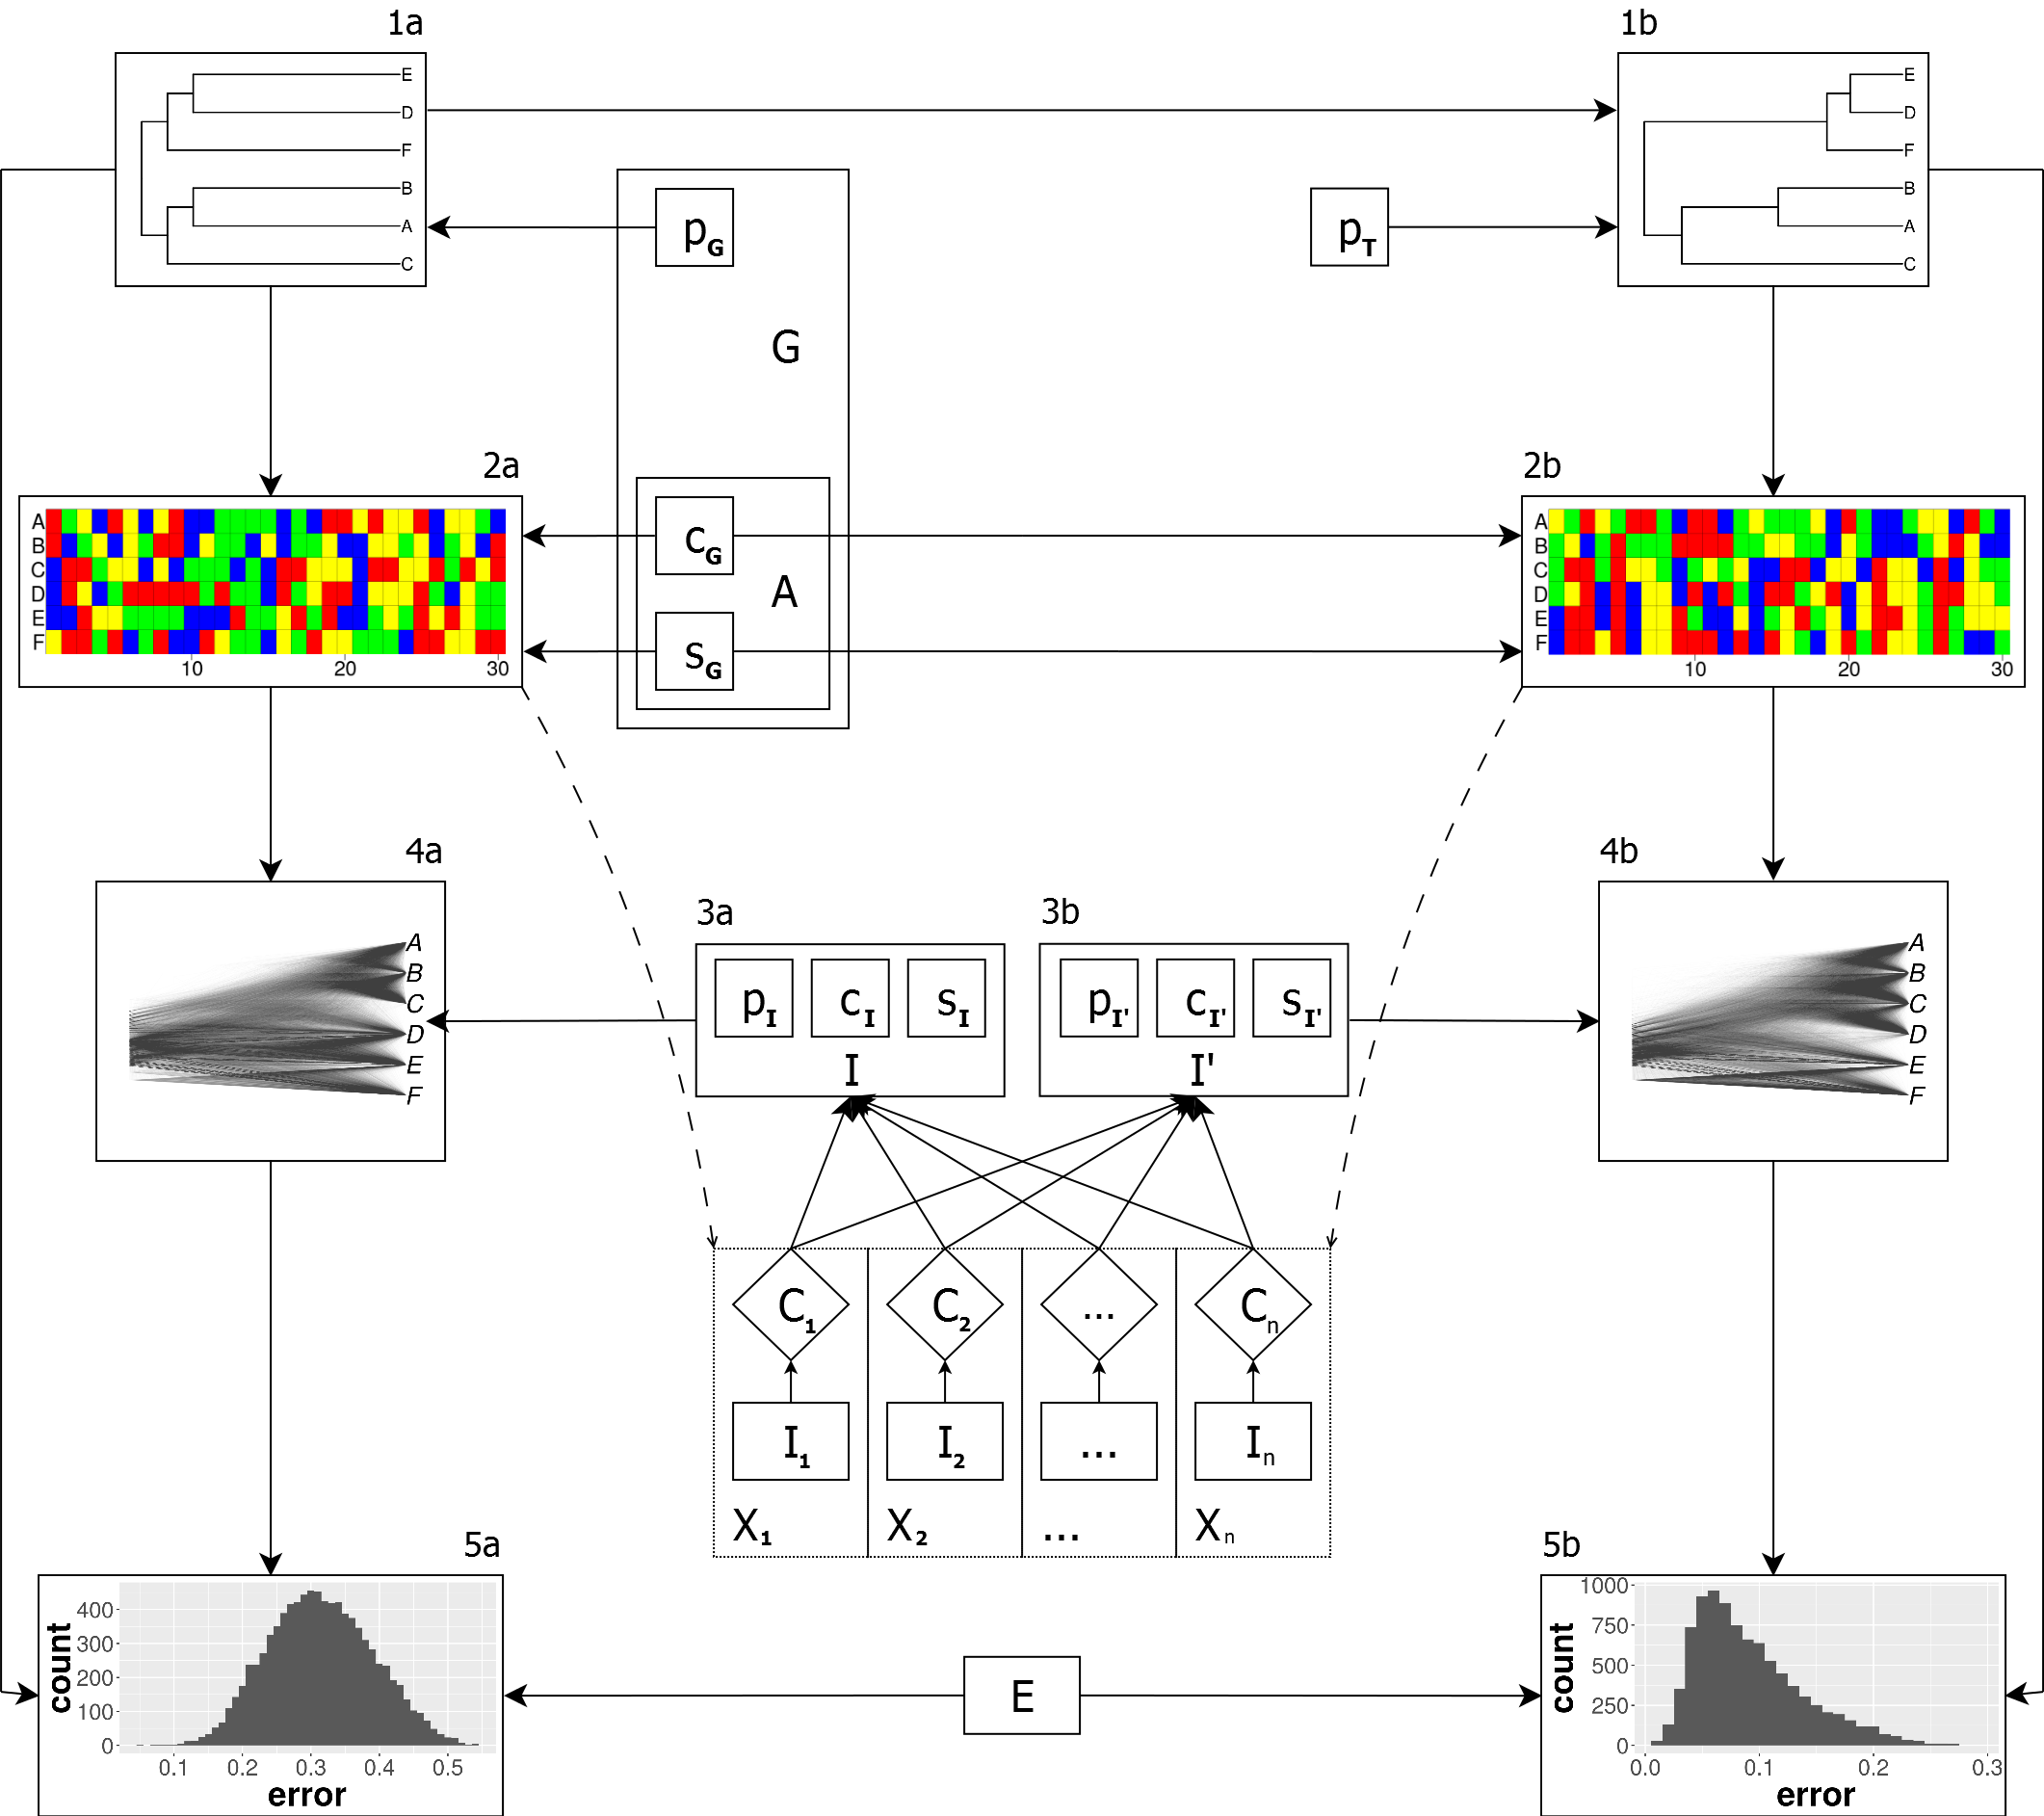
\includegraphics[width = \textwidth]{workflow4.png}
  \caption{
    \texttt{pirouette} pipeline.
    The pipeline starts from a phylogeny (1a) simulated by the generative tree model 
    $\mathit{p_{G}}$.
    The phylogeny is converted to an alignment (2a) using the generative alignment model 
    $\mathit{A} = (\mathit{c_{G}}, \mathit{s_{G}})$, composed of a clock and a site model. 
    The user defines one or more experiments.
    For each candidate experiment $\mathit{X_{i}}$ 
    (a combination of inference model $\mathit{I_{i}}$ and condition $\mathit{C_{i}}$),
    if its condition $\mathit{C_{i}}$ is 
    satisfied (which can depend on the alignment), 
    the corresponding inference model $\mathit{I} = \mathit{I_{i}}$ is selected
    to be used in the next step.
    The inference models (3a) of the selected experiments use the alignment (2a) 
    to each create a Bayesian posterior of (parameter estimates and) 
    phylogenies (4a). 
    Each of the posteriors' trees is compared to the true phylogeny (1a) 
    using the error measure $\mathit{E}$, 
    resulting in an error distribution (5a). 
    Optionally, for each selected inference model a twin pipeline can be run.
    A twin phylogeny (1b) can be generated from the original 
    phylogeny (1a) using the twin tree model $\mathit{p_{t}}$, 
    selected among standard diversification models; 
    the default option is the standard BD model, 
    with parameters estimated from the original phylogeny.
    A twin alignment (2b) is then simulated from the twin phylogeny 
    using clock model $\mathit{c_{G}}$ and site model $\mathit{s_{G}}$ 
    imported from the generative model. 
    The twin alignment has the same number of mutations as the original alignment.
    The twin pipeline follows the procedure of the main pipeline, 
    resulting in a twin error distribution (5b).
  }
  \label{fig:pipeline}
\end{figure}

The pipeline to assess the error BEAST2 makes in inferring this phylogeny 
then contains the following steps:
\begin{enumerate}
  \item the user supplies one or (ideally) more phylogenies from a 
    new diversification model
  \item from the given phylogeny an alignment is simulated 
    under a known alignment model $\mathit{A}$;
  \item from this alignment, according to the specified 
    inference conditions $\mathit{C}$, 
    an inference model $\mathit{I}$ is chosen (which may differ from the 
    generative model);
  \item the inference model and the alignment are used 
    to infer a posterior distribution of phylogenies;
  \item the phylogenies in the posterior are compared with the given phylogeny 
    to estimate the error made, according to 
    the error measure $\mathit{E}$ specified by the user;
\end{enumerate}

The pipeline is visualized in Fig.~\ref{fig:pipeline}. 
There is also the option to generate a 'twin tree', 
that goes through the same pipeline. 
The utility of this twin tree will be explained below.

The first step simulates an alignment from the given 
phylogeny (Fig.~\ref{fig:pipeline}, 1a $\rightarrow$ 2a).
For the sake of clarity, here we will assume the alignment consists out
of DNA sequences, but other heritable material such as amino acids also works.
The user must specify a root sequence, a mutation rate and a site model.
The root sequence is the DNA sequence of the shared common ancestor,
and is set to four different equally-sized mononucleotide blocks by default, 
which helps interpreting the resulting alignment.
Supported nucleotide substitution models (part of a DNA
site model) are JC, HKY, TN and GTR (see \ref{tab:options} for
the meaning of these abbreviatons).
JC is the default nucleotide subsitution mode (NSM),
in which the nucleotide substition rates between all
nucleotides are equal and constant over time.
Note that the user cannot specify a clock model, as only the strict clock model 
is implemented and thus always assumed.

The second step (Fig.~\ref{fig:pipeline}, 3a)
selects one (or more) inference model(s) $I$ from a set of inference models $I_{1},\dots,I_{n}$. 
We define an experiment $X_{i}$ as the combination of 
an inference model $I_{i}$ and the conditions $C_{i}$ 
to actually use it in the inference step.
For example, we may require that an inference
model (a combination of a tree model, clock model and site model) 
should include the generative/true tree model. 
As a second example, we may require that we have selected a set of 
candidate inference models,
of which only the best should be used in the actual inference.
In the first example, we specified the condition $C_{i}$ that this
generative model should always be run, whereas in the second example,
we specified condition $C_{i}$ that a candidate model should only be run
when it is the best.
The 'best' model is defined as the inference model with
the highest evidence (a.k.a. marginal likelihood), based on the alignment 
simulated in the previous step.
The evidence for an inference model is estimated by nested 
sampling [\cite{russel2019model}], using the \verb;NS; BEAST2 package. 
We note that scripted use of BEAST2 packages is only possible under Linux and Mac.
Windows systems can do the model comparison for shorter DNA sequences 
using the web interface of \verb;mcbette; [\cite{mcbette}].

The third step infers the posterior distributions,
using the simulated alignment (Fig.~\ref{fig:pipeline}, 2a $\rightarrow$ 4a),
and the inference models that were selected in the previous step (3a). 
For each selected experiment a posterior distribution is inferred, using the 
\verb;babette; [\cite{bilderbeek2018babette}] R package which makes use of BEAST2. 
This step usually takes up most of the pipeline's computation time.

The fourth step quantifies the inference error made. 
First the burn-in fraction is removed, i.e. the first phase of the 
Markov chain Monte Carlo (MCMC) run,
which samples an unrepresentative part of state space. 
By default, \verb;pirouette; 
removes the first 10\% of the posterior.
From the remaining posterior \verb;pirouette; 
creates an error distribution, by measuring the difference
between the true tree and each of the posterior 
trees (Fig.~\ref{fig:pipeline}, 4a $\rightarrow$ 5a).
The user can specify a function to quantify the differences between
the true and posterior trees. By default, the package uses the nLTT 
statistic (\cite{janzen2015approximate}), which is the absolute difference
between the normalized lineages-through-time plots of two trees.
The nLTT statistic is chosen, as it can operate on any two trees (regardless
of their crown ages and number of taxa) and its results have a clear range
from zero to one. This normalized result makes it possible to compare trees 
from a distribution of trees from any tree model.

\subsection{Twinning}\label{subsec:twinning}

An optional step is to use the 'twinning process'.
This process, $T$, encompasses two steps:
$T_1$, that generates a 'twin tree' (Fig.~\ref{fig:pipeline}, 1b) 
and $T_2$, which generates a 'twin alignment' (Fig.~\ref{fig:pipeline}, 2b).
Both twin tree and alignment will be analyzed in the same way 
as the true tree and alignment.

We define a phylogeny $\tau$ as the combination of
branching times $\Vec{t}$ and topology $\psi$, 
and denote as $\tau_{\mathit{G}}$ the phylogeny 
produced by a (possibly non-standard) generative diversification model, 
having branching times $\Vec{t}_{\mathit{G}}$ and 
topology $\psi_{\mathit{G}}$.

The first step ($T_1$) of the twinning process creates a tree $\tau_{\mathit{T}}$
with branching times $\Vec{t}_{\mathit{T}}$ while preserving the original
topology $\psi_{\mathit{G}}$:
\begin{align}
  \tau_{\mathit{G}} = (\Vec{t}_{\mathit{G}}, \psi_{\mathit{G}}) 
  \xrightarrow[]{\mathit{T_1}} 
  \tau_{\mathit{T}} = (\Vec{t}_{\mathit{T}}, \psi_{\mathit{G}})
\end{align}
The default option for the diversification model $p_T$ is the standard BD model.
It is then possible to use the likelihood function 
$L_{\mathit{T}}$ for this diversification model to find the parameters $\theta^{*}_{\mathit{T}}$ 
(e.g. speciation and extinction rates, in case of a BD model) 
that maximize this likelihood applied 
to the true tree, conditioned on its number of tips $n_{\mathit{G}}$:
\begin{align}
    \max[L_{\mathit{T}}(\theta_{\mathit{T}}|\tau_{\mathit{G}}, n_{\mathit{G}})] 
\rightarrow \theta^{*}_{\mathit{T}}.
\end{align}
We use $\theta^{*}_{\mathit{T}}$ to simulate a number 
$n_{\mathit{T}} = n_{\mathit{G}}$ 
of branching times $\Vec{t}_{\mathit{T}}$ for the twin tree 
$\tau_{\mathit{T}}$, under the process $p_{T}$, 
while preserving the topology. 
We simulate the new branching times using the TESS package (\cite{TESS, hohna2016tess}).

The second step ($T_2$) of the twinning process simulates the twin alignment 
with the same clock model, site model and mutation rate 
used to simulate the original alignment. 
We also impose that, in the twin alignment, 
the total number of mutations with respect to the root sequence 
must be the same as in the true alignment in order to keep the information content 
stored in both the true and twin alignments as similar as possible. 
We achieve this by simply simulating twin alignments until we
obtain one that has the desired number of mutations.

The twin pipeline serves as a control: 
even when the generating and inference models are identical
(as is the case in the twin pipeline),
the inferred trees from the posterior distribution will 
still differ from the true tree, 
due to stochasticity in producing an alignment 
and to the MCMC sampling of the posterior.
The twin pipeline provides this minimum error,
because the generating and inference model match exactly.
When comparing the true and twin error distribution,
any differences will be due to the fact that true and twin phylogenies are realizations 
of different processes: one (possibly) non-standard, $p_G$, 
and one standard, $p_T$ (see Fig~\ref{fig:pipeline}).

This can be seen for both the "generative" and "candidate" model 
types (see Table~\ref{tab:options}).
If the chosen model type is "generative", 
the tree prior chosen for the twin inference will  
exactly match the model to generate the tree.
In the main pipeline, as the tree model $p_{G}$ is non-standard, 
it cannot be used in inference.
If, instead, the chosen model type is "candidate", 
the twin tree model will be included in the pool of examined models 
during the process of selection of the inference model. 

Finally, if the goal is to evaluate BEAST2's performance on a non-standard tree prior, 
one must also consider the last source of stochasticity: 
the different phylogenies a tree model generates.
A single phylogeny cannot be considered as fully representative of the model. 
For this reason multiple phylogenies, as well as an equal number of twins, must be considered. 
If the number of considered phylogenies is high enough, 
the comparison between the main pipeline's aggregated error distribution 
and its twin counterpart leads to a fair evaluation 
of the new tree prior with respect to the baseline error.

%%%%%%%%%%%%%%%%%%%%%%%%%%%%%%%%%%%%%%%%%%%%%%%%%%%%%%%%%%%%%%%%%%%%%%%%%%%%%%%%
\section{Usage}
%%%%%%%%%%%%%%%%%%%%%%%%%%%%%%%%%%%%%%%%%%%%%%%%%%%%%%%%%%%%%%%%%%%%%%%%%%%%%%%%

We show the usage of \verb;pirouette; on an tree generated 
by the non-standard diversity-dependent tree model \cite{DDD, etienne2011diversity},
which is a birth-death model with a speciation rate that is dependent on the number of species. 

We use a small tree with six taxa, to keep the figure more readable,
with an arbitrary crown age of ten time units.

\begin{figure}[H]
  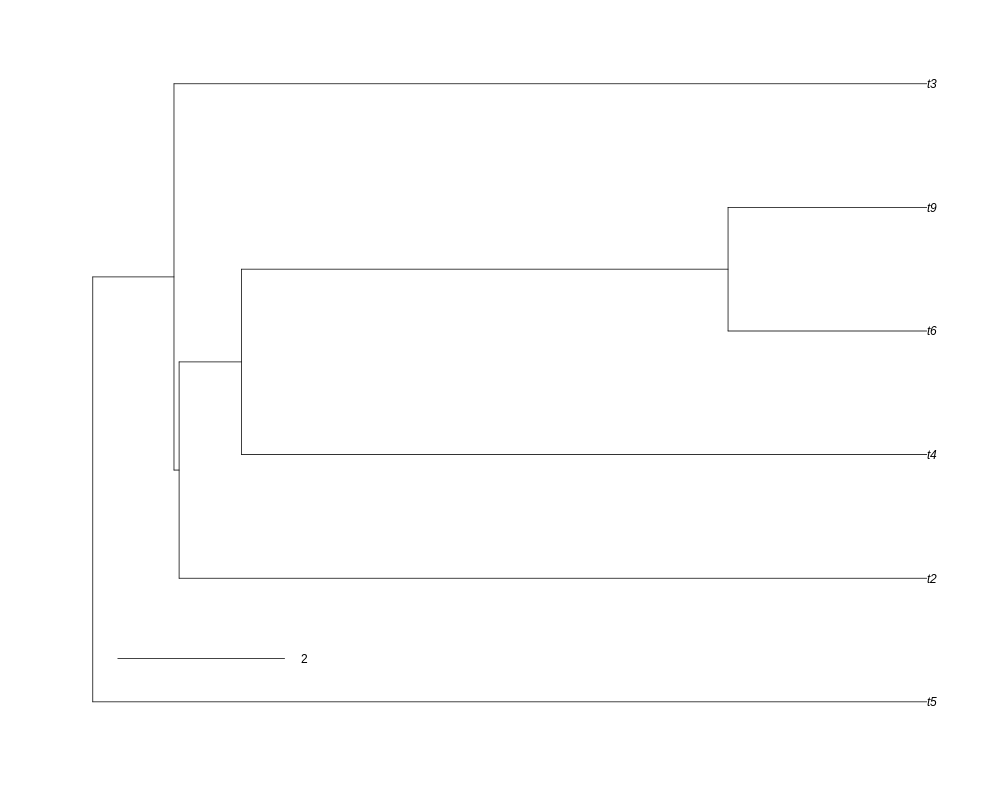
\includegraphics[width=\textwidth]{pirouette_example_30/example_30_314/true_tree.png}
  \caption{
    The tree derived from a DD process, 
    as created by listing~\ref{lst:create_dd_tree}.
  }
\end{figure}

The first step in \verb;pirouette; is to 
simulate a DNA alignment from the 
given phylogeny, as described in Subsection~\ref{subsec:pipeline}.
In this example, the root sequence consists of four blocks of 250 
mononucleotides each, while the per-nucleotide mutation rate is 
0.1 mutations per unit time.
Together with the crown age of 10 time units, this results
in an expected per-locus mutation probability of 1.
We use a Jukes-Cantor (JC, \cite{jukes1969evolution}) NSM
and a strict clock model as these are the simplest.
A JC model assumes that mutation rates between nucleotides are equal and 
constant. 
A strict clock model assumes that the mutation rates 
of all lineages are equal and constant.

In the second step we state our experiment.
We define an experiment $\mathit{X}$ 
as a combination of an inference model 
$\mathit{I}$ and conditions $\mathit{C}$.
As a generative model, we assume a
site model with a JC69 NSM,
a strict clock model and a Yule tree prior.
For our candidate models,
we select all 16 experiments
that are a combination of the 4 NSMs,
2 clock models and 2 BD tree priors.
From this set, we exclude the generative model.

We use the nLTT statistic to
measure the difference between phylogenies,
with a burn-in of 10\%.

\begin{figure}[H]
  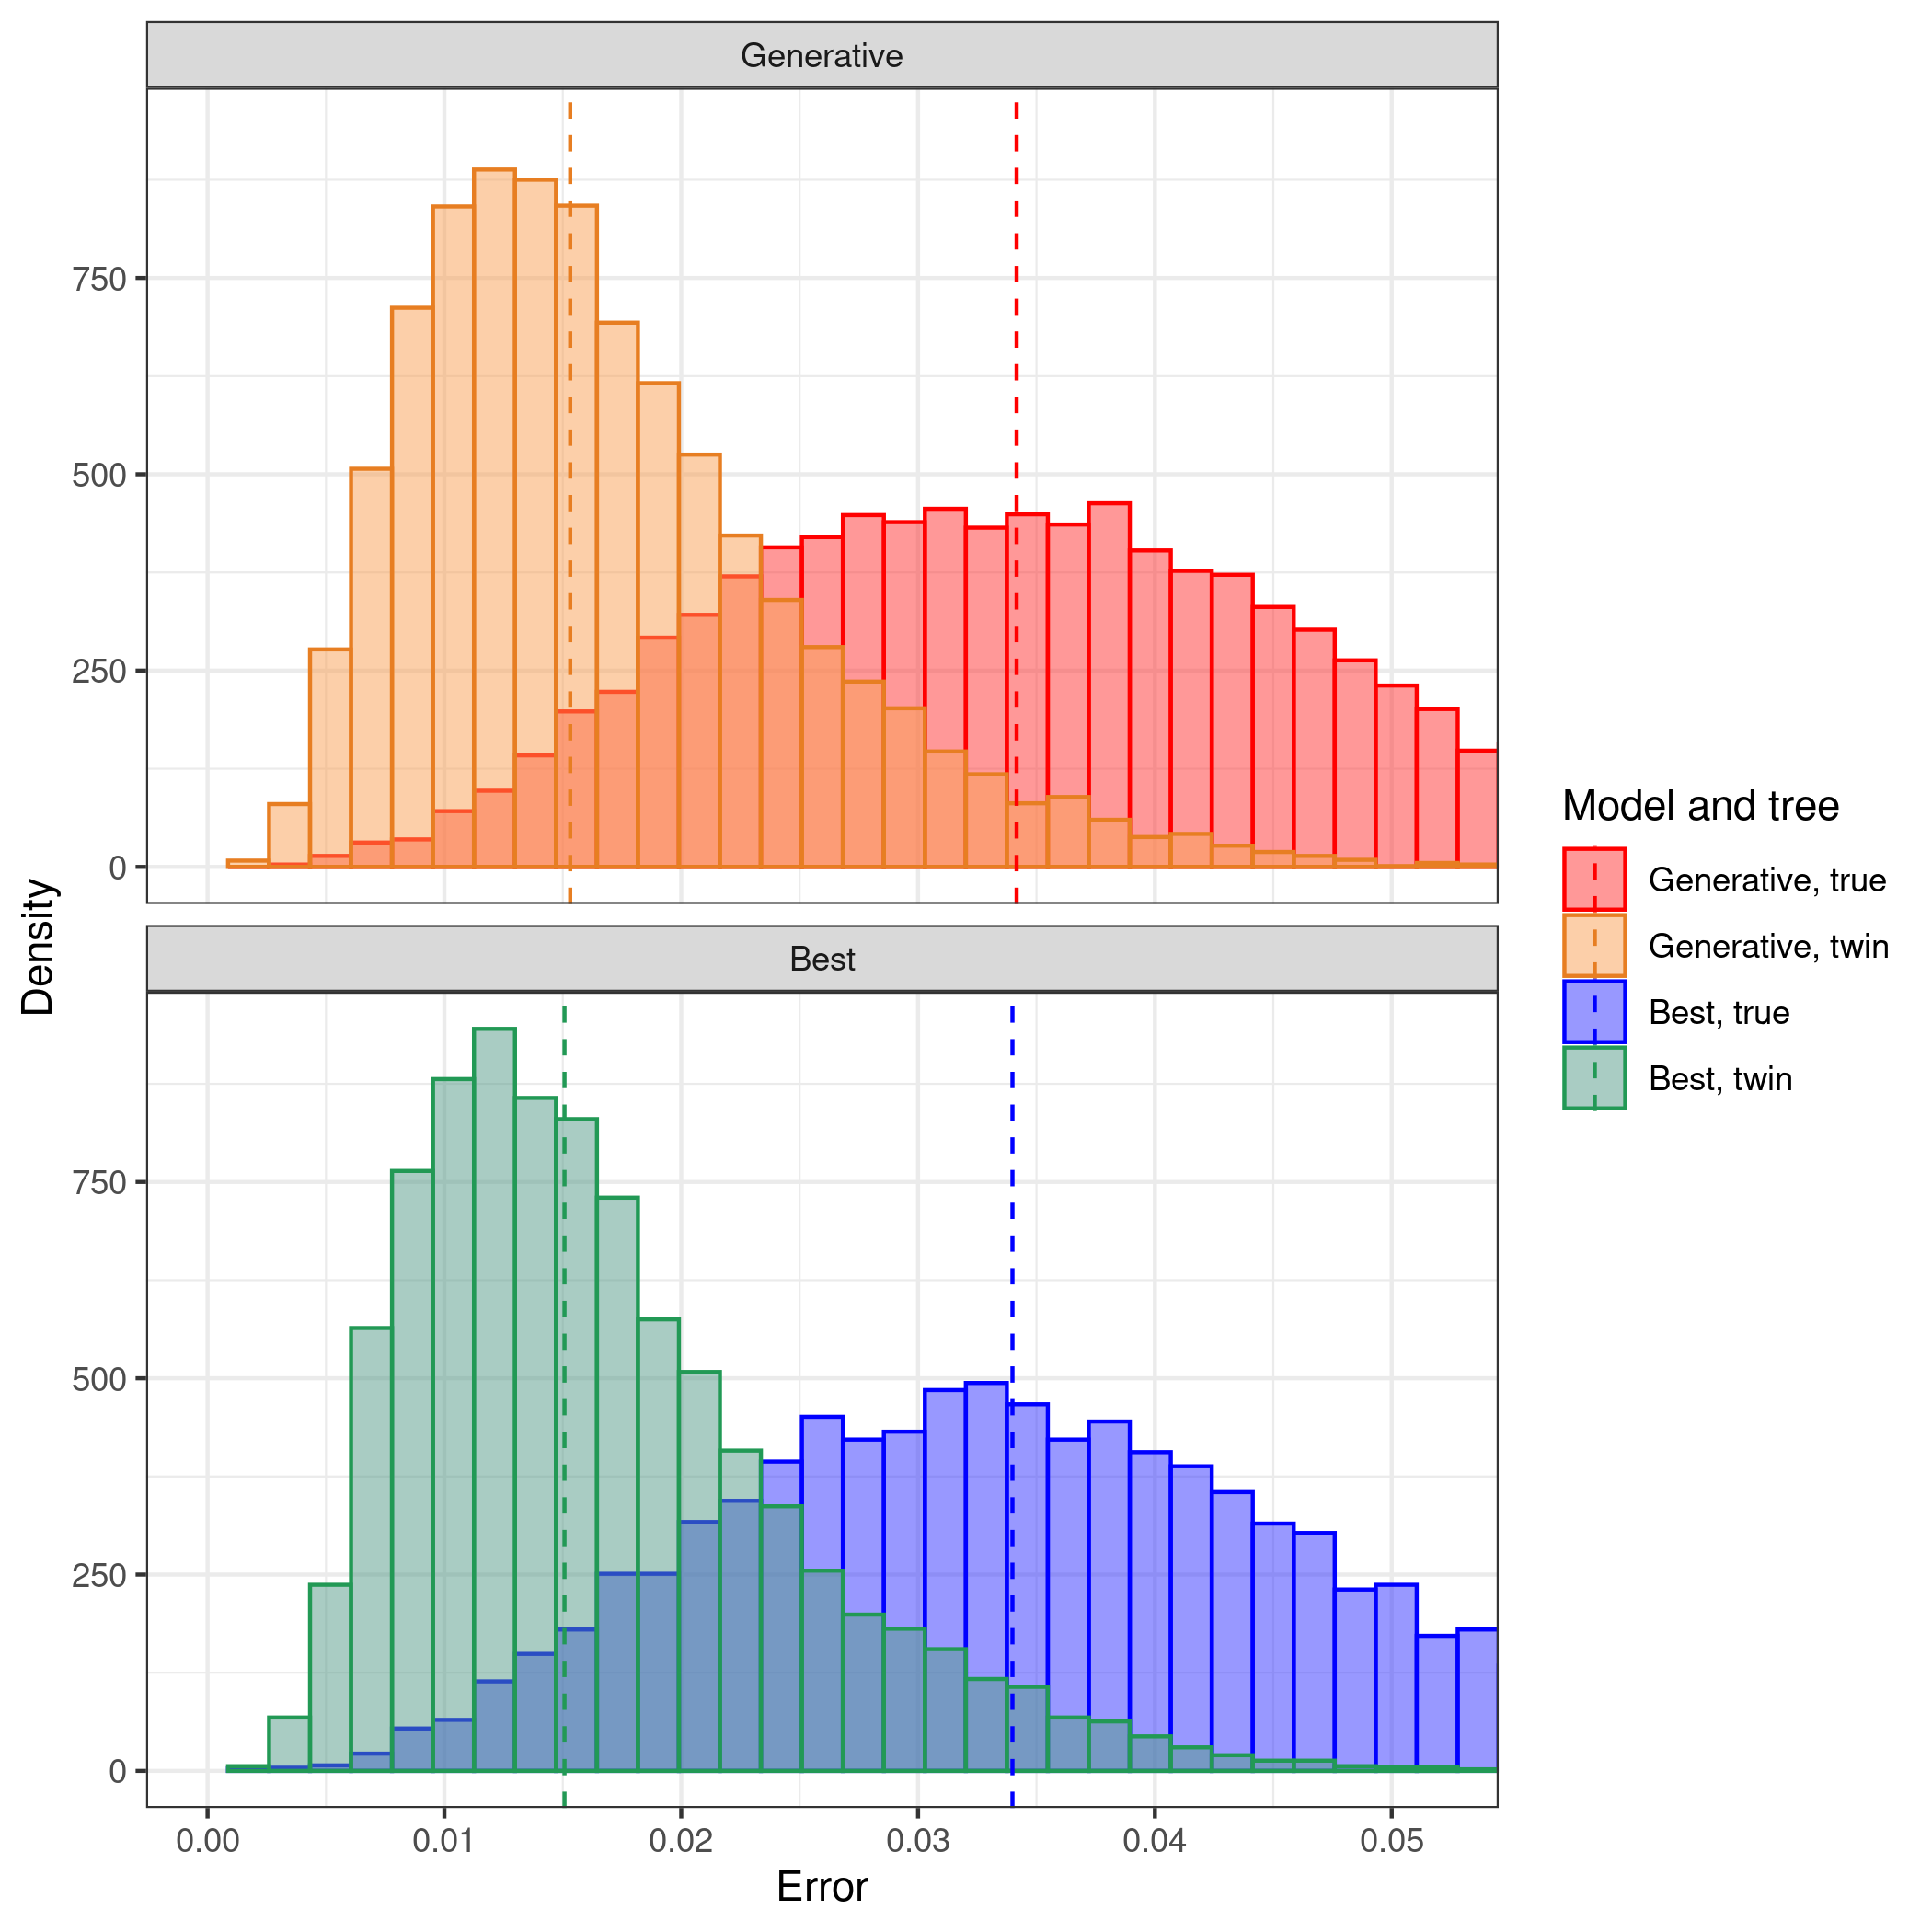
\includegraphics[width=\textwidth]{pirouette_example_30/errors.png}
  \caption{
    The inference error made 
    for both a generative tree prior and best candidate model
    compared with the error obtained for the twin tree.
    Here, the 'twin' tree shows the baseline inference error.
    Vertical dashed lines show the median error value per distribution.
  }
  \label{fig:example_30}
\end{figure}

While the error distributions using the best or generative model 
as inference model are very similar, 
the error distributions of the true tree are substantially 
larger than those of the twin tree. 
This is the error made by the mismatch
between the generating species tree model and the tree prior used in inference.

%%%%%%%%%%%%%%%%%%%%%%%%%%%%%%%%%%%%%%%%%%%%%%%%%%%%%%%%%%%%%%%%%%%%%%%%%%%%%%%%
\section{Discussion}
%%%%%%%%%%%%%%%%%%%%%%%%%%%%%%%%%%%%%%%%%%%%%%%%%%%%%%%%%%%%%%%%%%%%%%%%%%%%%%%%

We showed how to use \verb;pirouette; to quantify the importance of a 
tree prior in Bayesian phylogenetics, using the simplest generative tree 
model possible.
In principle any other (more complex) generative tree model can be tested, 
but we chose to provide the simplest (and fastest to run) examples.

Figure~\ref{fig:example_3} illustrates the primary result of our pipeline: 
it shows the error distributions for the true tree and the twin tree 
when either the generating model or the best candidate model is used in inference. 
The clear difference between the error distributions 
for the true tree and the twin tree suggests 
that the choice of tree prior does matter.

We note, however, that all examples used only one original tree,
where any speciation process produces a whole range of trees.
One tree is not enough to determine the impact 
of a tree prior on Bayesian inference.
However, if the same procedure were repeated and 
performed on a distribution with a sufficient number of generative trees, 
it would constitute a quantitative and effective assessment of the 
quality of the inference.
Also a twin tree does not always result in a lower error distribution,
as the stochasticity in generating a twin tree will - with
very low probability - yield a tree of that same very low probability.

In conclusion, \verb;pirouette; can show the errors to be expected
when the tree prior used in inference is different from the generating model.
The user can then judge whether or not a new tree prior, 
tailored on the generative process, is needed. 
If this is indeed the case, one can implement the novel tree prior as an addition to 
his/her favorite Bayesian inference tool.

%%%%%%%%%%%%%%%%%%%%%%%%%%%%%%%%%%%%%%%%%%%%%%%%%%%%%%%%%%%%%%%%%%%%%%%%%%%%%%%%
\section{pirouette resources}
%%%%%%%%%%%%%%%%%%%%%%%%%%%%%%%%%%%%%%%%%%%%%%%%%%%%%%%%%%%%%%%%%%%%%%%%%%%%%%%%

\verb;pirouette; is free, libre and open source software available at 
\url{http://github.com/richelbilderbeek/pirouette},
licensed under the GNU General Public License version 3.
\verb;pirouette; depends on multiple packages, which are:
\verb;ape; (\cite{ape}),
\verb;babette; (\cite{bilderbeek2018babette}),
\verb;becosys; (\cite{becosys}),
\verb;DDD; (\cite{DDD}),
\verb;devtools; (\cite{devtools}),
\verb;dplyr; (\cite{dplyr}),
\verb;geiger; (\cite{geiger}),
\verb;ggplot2; (\cite{ggplot2}),
\verb;knitr; (\cite{knitr}),
\verb;lintr; (\cite{lintr}),
\verb;magrittr; (\cite{magrittr}),
\verb;mcbette; (\cite{mcbette}),
\verb;nLTT; (\cite{nLTT}),
\verb;PBD; (\cite{PBD}),
\verb;phangorn; (\cite{phangorn}),
\verb;phytools; (\cite{phytools}),
\verb;plyr; (\cite{plyr}),
\verb;rappdirs; (\cite{rappdirs}),
\verb;rmarkdown; (\cite{rmarkdown}),
\verb;Rmpfr; (\cite{Rmpfr}),
\verb;stringr; (\cite{stringr}),
\verb;TESS; (\cite{TESS}),
\verb;testit; (\cite{testit}), 
\verb;testthat; (\cite{testthat}) and
\verb;tidyr; (\cite{tidyr}).

\verb;pirouette;'s development takes place on GitHub,
\url{https://github.com/richelbilderbeek/pirouette},
which allows submitting bug reports, requesting features, 
and adding code. To ensure a high quality, \verb;pirouette; 
uses a continuous integration service, has a code coverage of above 95\%
and enforces the most commonly used R style guide (\cite{style_guide}).

\verb;pirouette;'s is extensively documented on its website,
its documentation and its vignettes.
The \verb;pirouette; website is a good starting point to learn
how to use \verb;pirouette;, as it links to tutorials and videos.
The \verb;pirouette; package documentation describes
all functions and liberally links to related functions.
All exported functions show a minimal example as part of their documentation.
The \verb;pirouette; vignette demonstrates extensively how 
to use \verb;pirouette; in a more informally written way. 

The code used in this article and more examples that are periodically 
tested, can be found at 
\url{https://github.com/richelbilderbeek/pirouette_examples}. 

%%%%%%%%%%%%%%%%%%%%%%%%%%%%%%%%%%%%%%%%%%%%%%%%%%%%%%%%%%%%%%%%%%%%%%%%%%%%%%%%
\section{Citation of pirouette}
%%%%%%%%%%%%%%%%%%%%%%%%%%%%%%%%%%%%%%%%%%%%%%%%%%%%%%%%%%%%%%%%%%%%%%%%%%%%%%%%

To cite \verb;pirouette; this article from within R, use:

\begin{lstlisting}[language=R]
> citation("pirouette")
\end{lstlisting}

%%%%%%%%%%%%%%%%%%%%%%%%%%%%%%%%%%%%%%%%%%%%%%%%%%%%%%%%%%%%%%%%%%%%%%%%%%%%%%%%
\section{Acknowledgments}
%%%%%%%%%%%%%%%%%%%%%%%%%%%%%%%%%%%%%%%%%%%%%%%%%%%%%%%%%%%%%%%%%%%%%%%%%%%%%%%%

We would like to thank the Center for Information Technology of the University 
of Groningen for its support and for providing access to the Peregrine 
high performance computing cluster. 
We thank the Netherlands 
Organization for Scientific Research (NWO) for financial support 
through a VICI grant awarded to RSE.

%%%%%%%%%%%%%%%%%%%%%%%%%%%%%%%%%%%%%%%%%%%%%%%%%%%%%%%%%%%%%%%%%%%%%%%%%%%%%%%%
\section{Data Accessibility}
%%%%%%%%%%%%%%%%%%%%%%%%%%%%%%%%%%%%%%%%%%%%%%%%%%%%%%%%%%%%%%%%%%%%%%%%%%%%%%%%

All code is archived at 
\url{http://github.com/richelbilderbeek/pirouette_article},
with DOI \url{https://doi.org/12.3456/zenodo.1234567}.

%%%%%%%%%%%%%%%%%%%%%%%%%%%%%%%%%%%%%%%%%%%%%%%%%%%%%%%%%%%%%%%%%%%%%%%%%%%%%%%%
\section{Authors' contributions}
%%%%%%%%%%%%%%%%%%%%%%%%%%%%%%%%%%%%%%%%%%%%%%%%%%%%%%%%%%%%%%%%%%%%%%%%%%%%%%%%

RJCB, GL and RSE conceived the idea for the package. 
RJCB created, tested and revised the package.
GL provided major contributions to the package.
RJCB wrote the first draft of the manuscript, 
GL and RSE contributed to revisions.

%%%%%%%%%%%%%%%%%%%%%%%%%%%%%%%%%%%%%%%%%%%%%%%%%%%%%%%%%%%%%%%%%%%%%%%%%%%%%%%%
% Bibliography
%%%%%%%%%%%%%%%%%%%%%%%%%%%%%%%%%%%%%%%%%%%%%%%%%%%%%%%%%%%%%%%%%%%%%%%%%%%%%%%%
% MEE style
\bibliographystyle{mee}
\bibliography{article}
%%%%%%%%%%%%%%%%%%%%%%%%%%%%%%%%%%%%%%%%%%%%%%%%%%%%%%%%%%%%%%%%%%%%%%%%%%%%%%%%



% Commmented out the next line for a quick recompile :+1:
%%%%%%%%%%%%%%%%%%%%%%%%%%%%%%%%%%%%%%%%%%%%%%%%%%%%%%%%%%%%%%%%%%%%%%%%%%%%%%%%
\section{Results in detail}
%%%%%%%%%%%%%%%%%%%%%%%%%%%%%%%%%%%%%%%%%%%%%%%%%%%%%%%%%%%%%%%%%%%%%%%%%%%%%%%%

%%%%%%%%%%%%%%%%%%%%%%%%%%%%%%%%%%%%%%%%%%%%%%%%%%%%%%%%%%%%%%%%%%%%%%%%%%%%%%%%
\subsection{Errors}
%%%%%%%%%%%%%%%%%%%%%%%%%%%%%%%%%%%%%%%%%%%%%%%%%%%%%%%%%%%%%%%%%%%%%%%%%%%%%%%%

%%%%%%%%%%%%%%%%%%%%%%%%%%%%%%%%%%%%%%%%%%%%%%%%%%%%%%%%%%%%%%%%%%%%%%%%%%%%%%%%
\subsection{Example 1}
%%%%%%%%%%%%%%%%%%%%%%%%%%%%%%%%%%%%%%%%%%%%%%%%%%%%%%%%%%%%%%%%%%%%%%%%%%%%%%%%

%%%%%%%%%%%%%%%%%%%%%%%%%%%%%%%%%%%%%%%%%%%%%%%%%%%%%%%%%%%%%%%%%%%%%%%%%%%%%%%%
\begin{figure}[ht]
  \centering
  \resizebox {0.8\columnwidth} {!} {
    \begin{tikzpicture}[
      ->,>=stealth',shorten >=1pt,auto,
      node distance=0.25\textheight, 
      semithick
    ]   
    \tikzstyle{every state}=[]
    \node[state, draw=none] (O) [] {
    };   
    \node[state] (A) [right of = O, rectangle] {
      \includegraphics[height=0.2\textheight]{example_1/true_tree.png}
    };   
    \node[state] (B) [below of = A, rectangle] {
      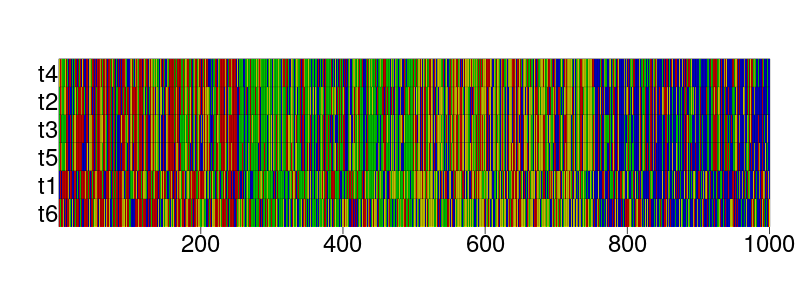
\includegraphics[height=0.2\textheight]{example_1/true_alignment.png}
    };   
    \node[state] (C) [below of = B, rectangle] {
      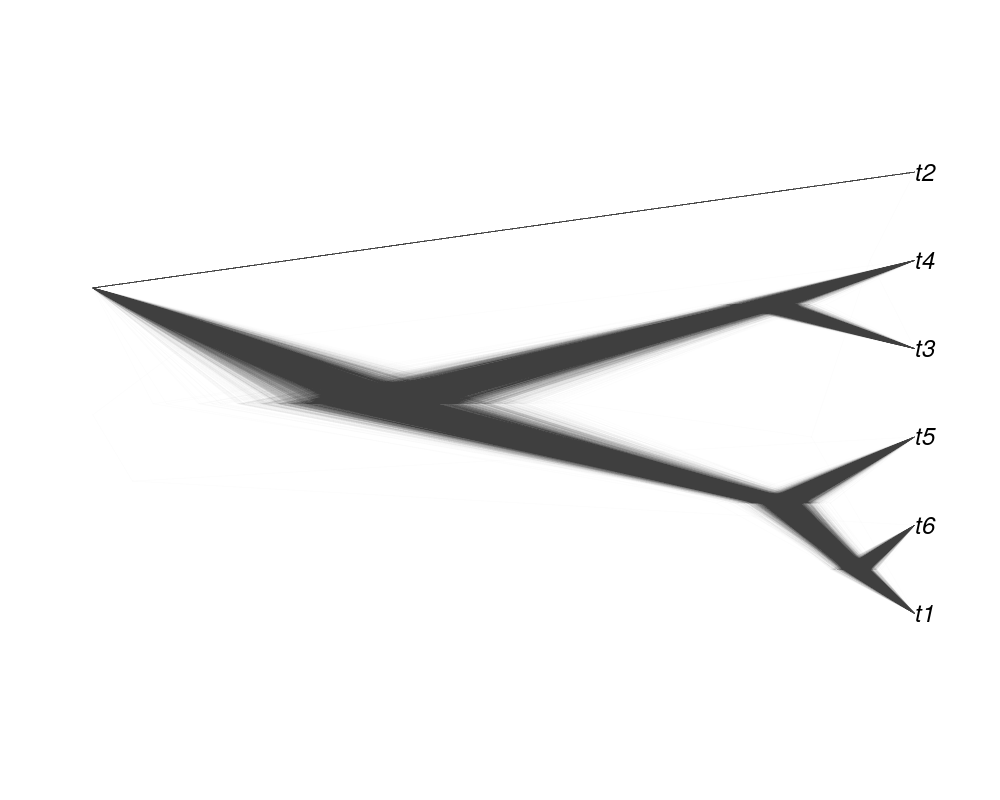
\includegraphics[height=0.2\textheight]{example_1/true_posterior_gen.png}
    };   
    \node[state] (D) [below of = C, rectangle] {
      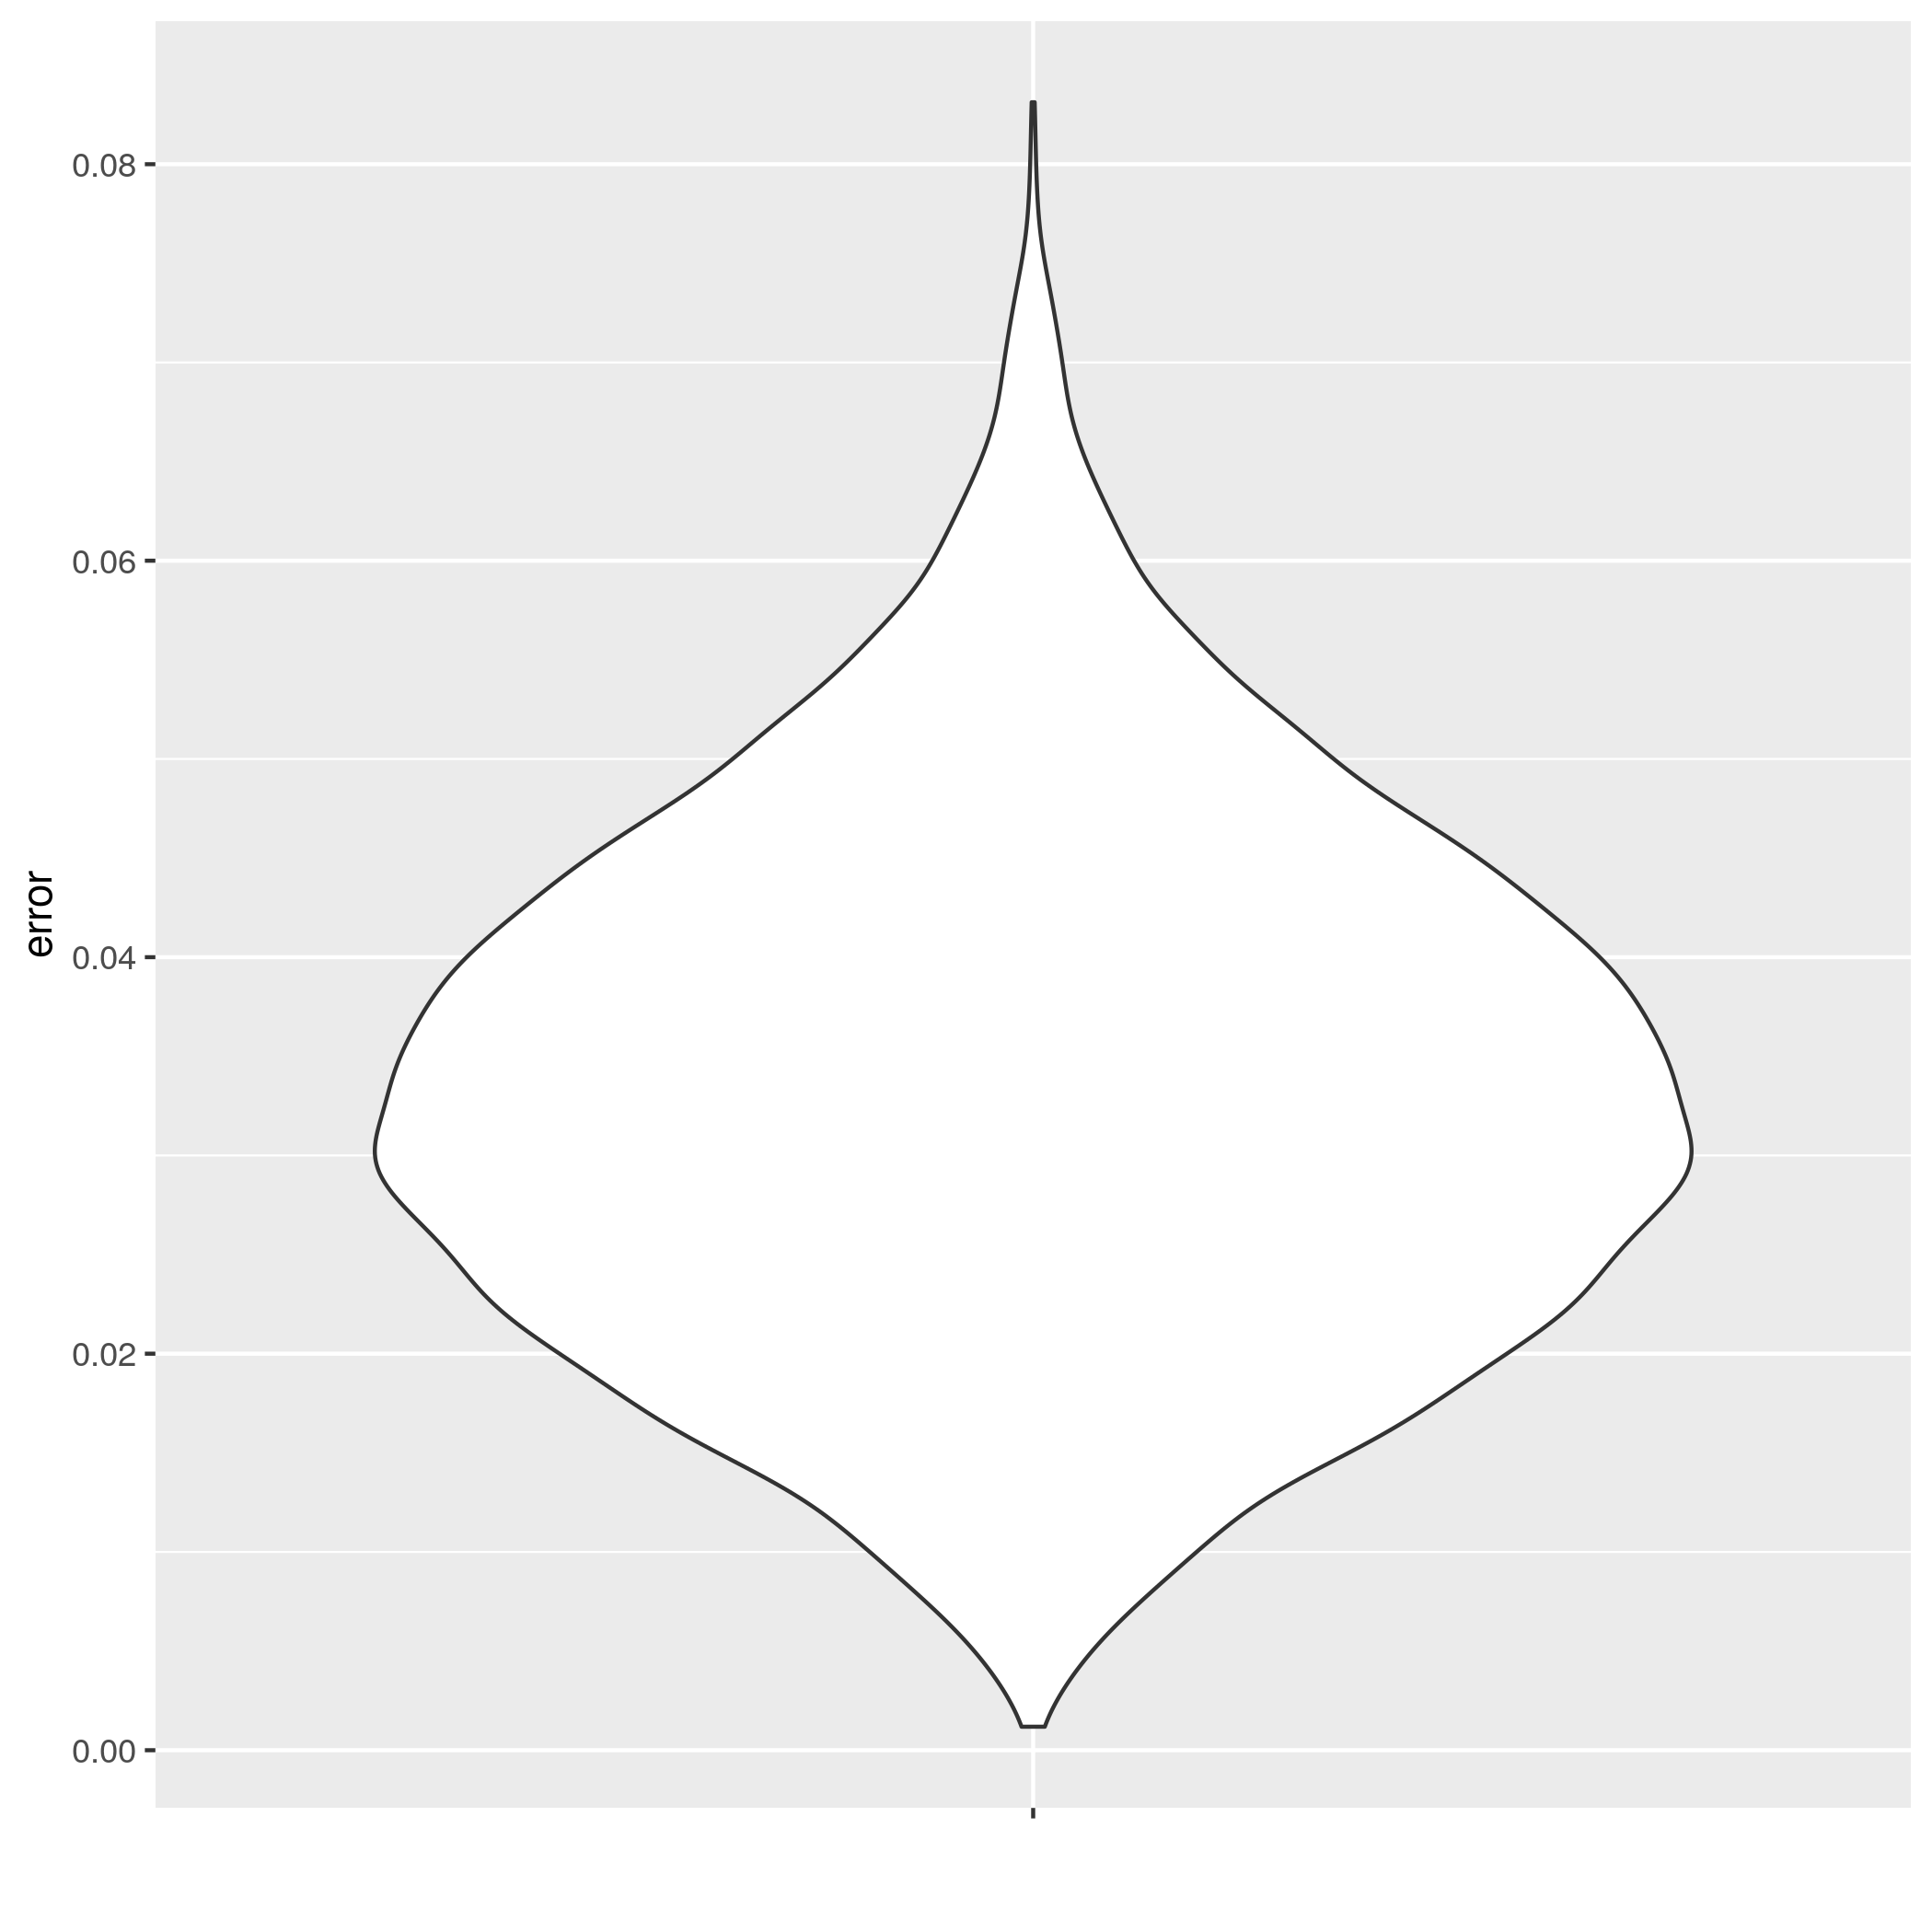
\includegraphics[height=0.2\textheight]{example_1/true_error_violin_gen.png}
    };   
    \path 
      (O) edge [anchor = south] node {} (A)
      (A) edge [anchor = south] node {} (B)
      (B) edge [anchor = south] node {} (C)
      (C) edge [anchor = south] node {} (D)
    ; 
    \end{tikzpicture}
  }
  \label{fig:example_1_full_pipeline}
  \caption{Example 1: full pipeline}
\end{figure}
%%%%%%%%%%%%%%%%%%%%%%%%%%%%%%%%%%%%%%%%%%%%%%%%%%%%%%%%%%%%%%%%%%%%%%%%%%%%%%%%

%%%%%%%%%%%%%%%%%%%%%%%%%%%%%%%%%%%%%%%%%%%%%%%%%%%%%%%%%%%%%%%%%%%%%%%%%%%%%%%%

\input{example_1/esses.latex}
% has label tab:esses_example_1

%%%%%%%%%%%%%%%%%%%%%%%%%%%%%%%%%%%%%%%%%%%%%%%%%%%%%%%%%%%%%%%%%%%%%%%%%%%%%%%%
\subsection{Example 5}
%%%%%%%%%%%%%%%%%%%%%%%%%%%%%%%%%%%%%%%%%%%%%%%%%%%%%%%%%%%%%%%%%%%%%%%%%%%%%%%%

%%%%%%%%%%%%%%%%%%%%%%%%%%%%%%%%%%%%%%%%%%%%%%%%%%%%%%%%%%%%%%%%%%%%%%%%%%%%%%%%
\begin{figure}[ht]
  \centering
  \resizebox {0.8\columnwidth} {!} {
    \begin{tikzpicture}[
      ->,>=stealth',shorten >=1pt,auto,
      node distance=0.4\textheight, 
      semithick
    ]   
    \tikzstyle{every state}=[]
    \node[state, draw=none] (O) [] {
    };   
    \node[state] (A) [right of = O, rectangle] {
      \includegraphics[height=0.2\textheight]{example_3/true_tree.png}
    };   
    \node[state] (B) [below of = A, rectangle] {
      \includegraphics[height=0.13\textheight]{example_3/true_alignment.png}
    };   
    \node[state] (CG) [below of = B, rectangle] {
      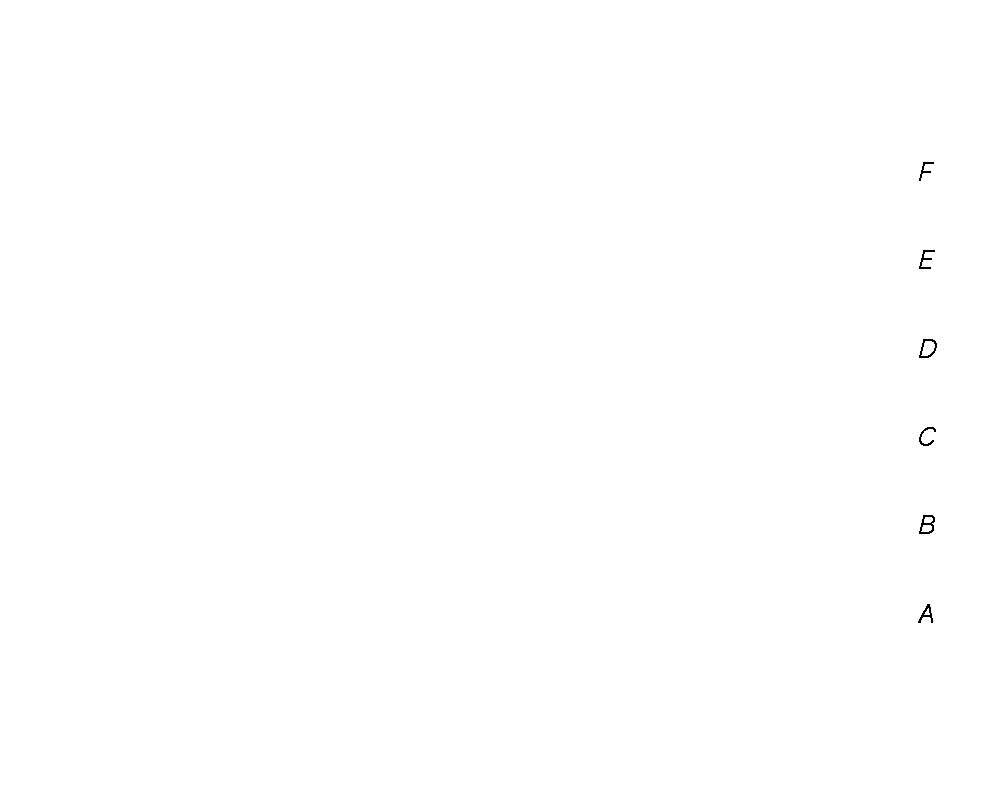
\includegraphics[height=0.2\textheight]{example_3/true_posterior_gen.png}
    };   
    \node[state] (DG) [below of = CG, rectangle] {
      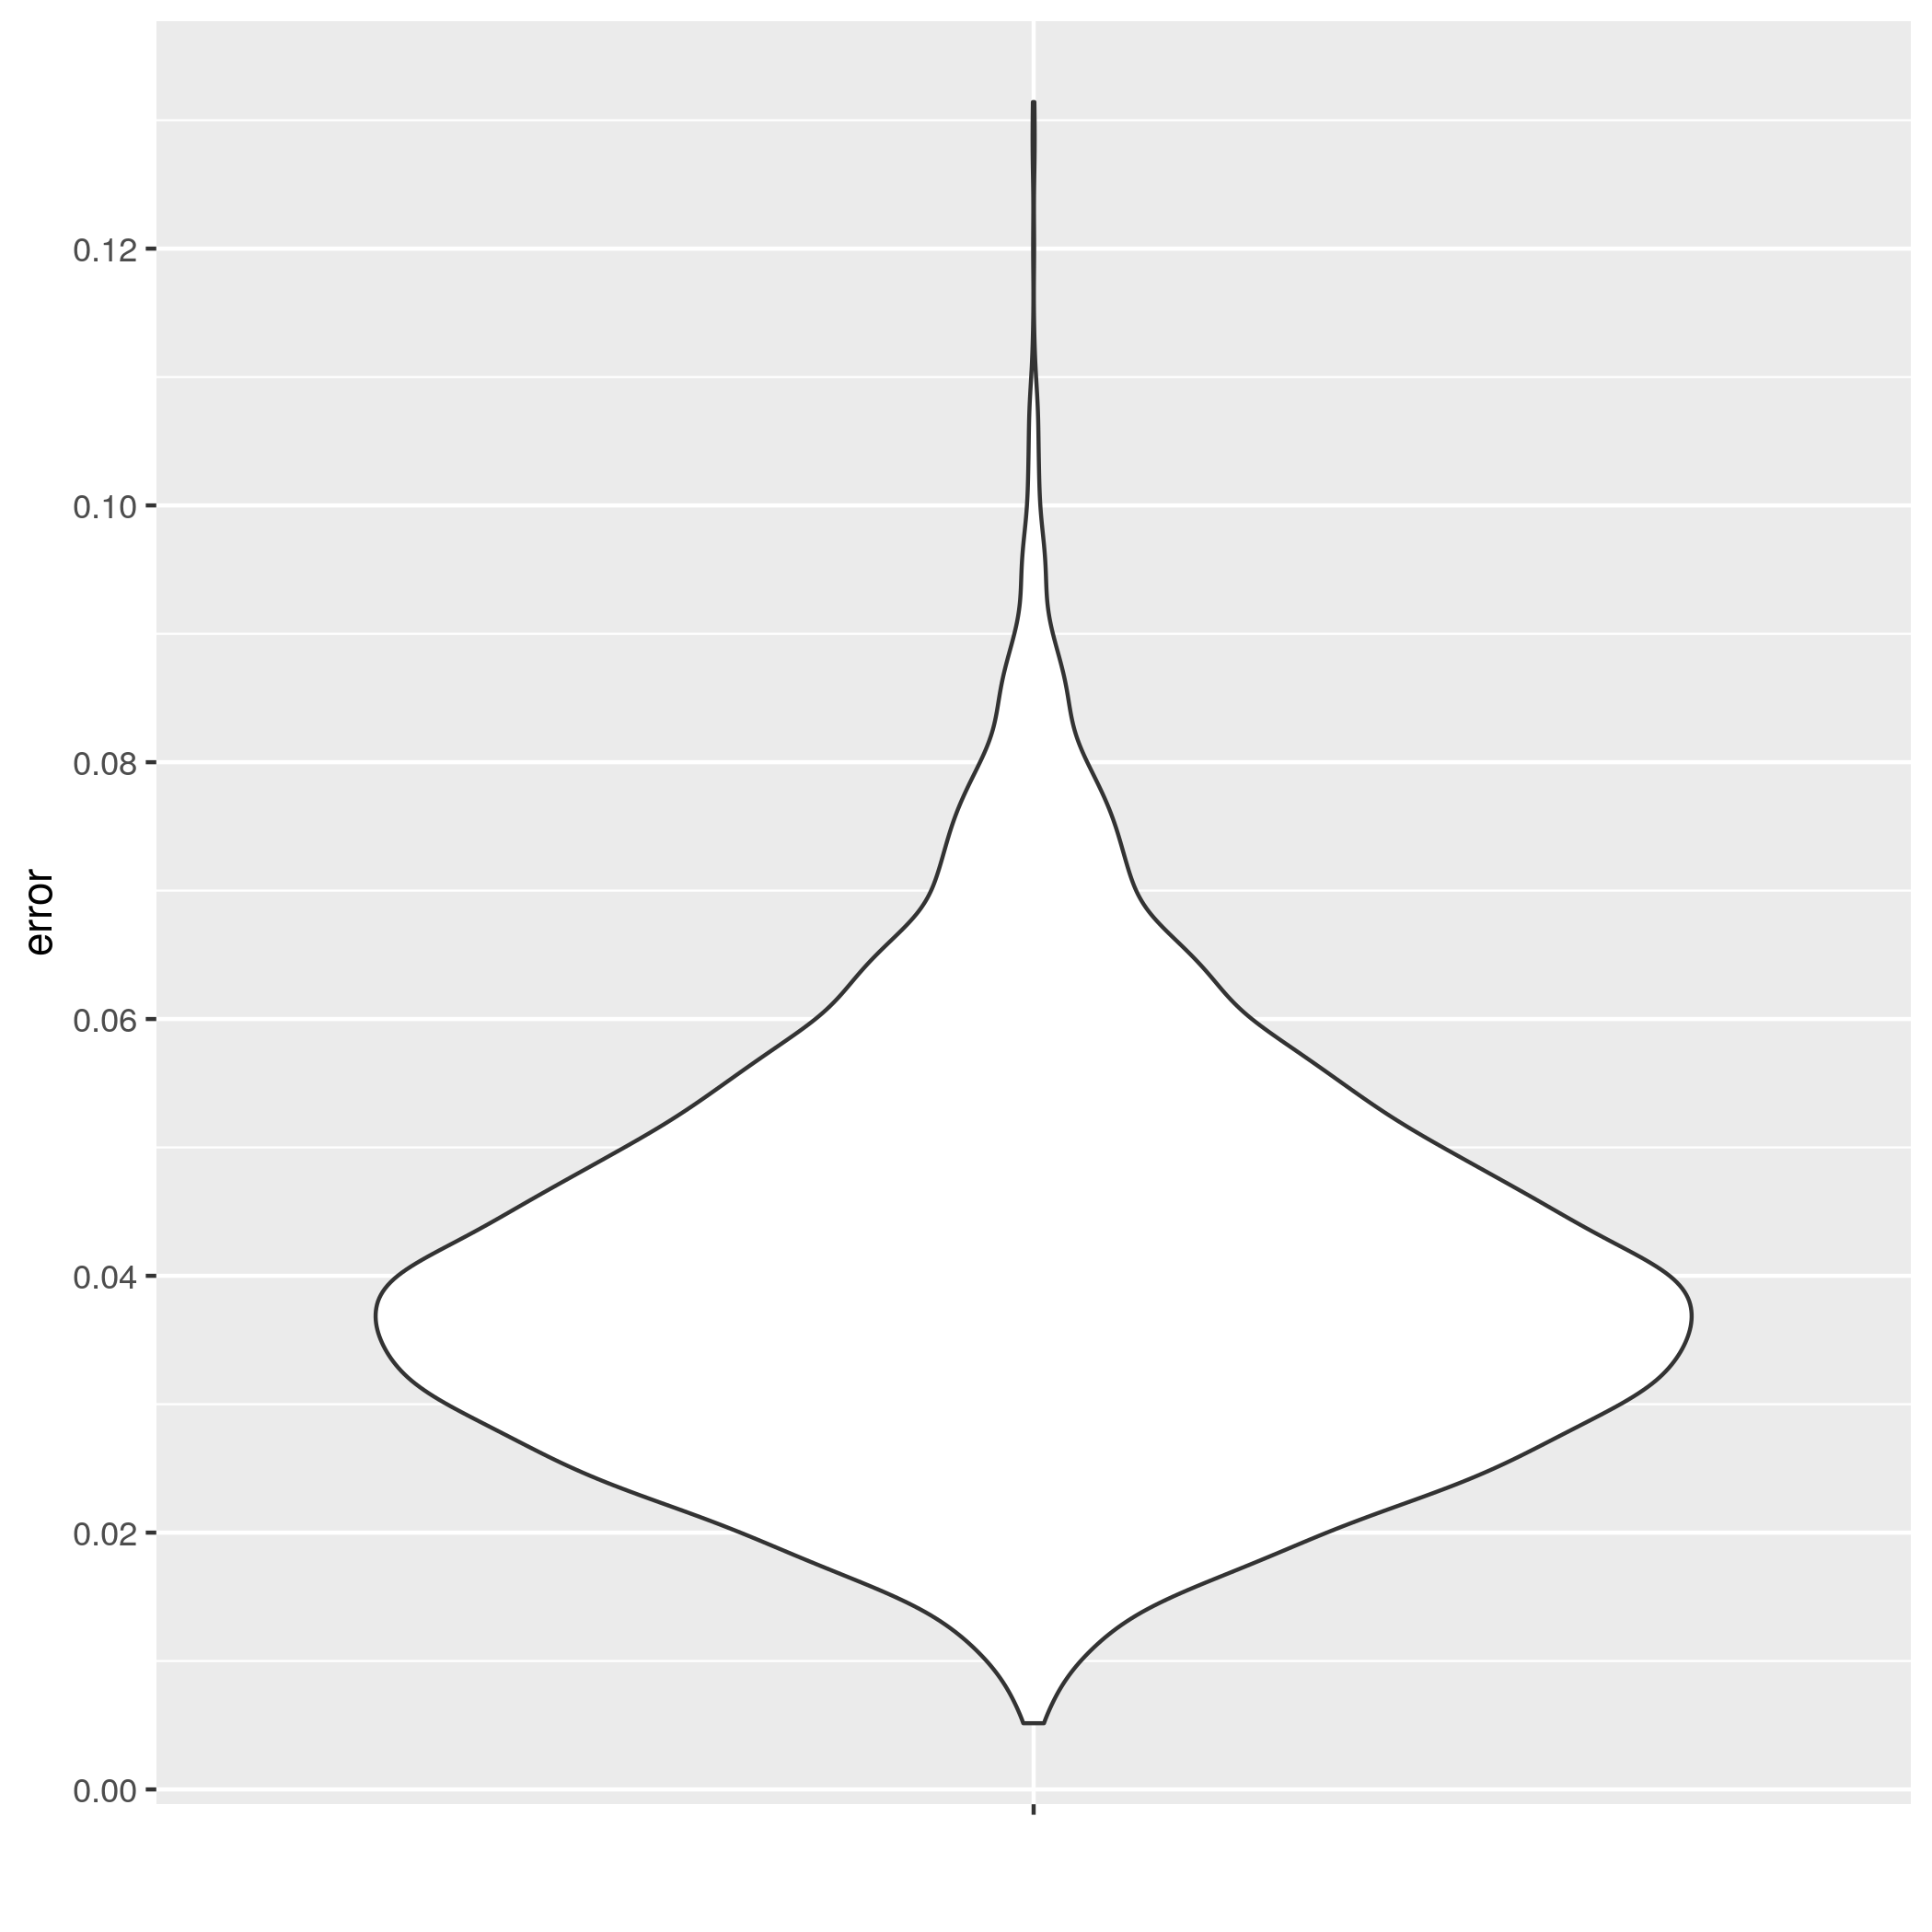
\includegraphics[height=0.2\textheight]{example_3/true_error_violin_gen.png}
    };   
    \node[state] (CB) [right of = C, rectangle] {
      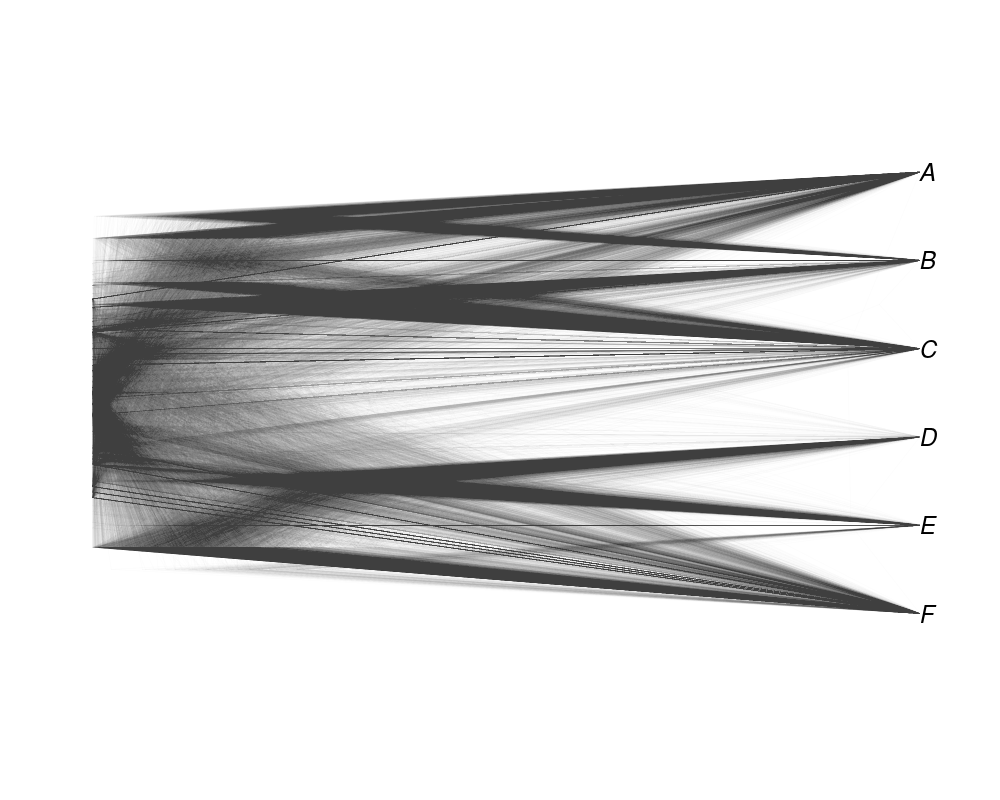
\includegraphics[height=0.2\textheight]{example_3/true_posterior_best.png}
    };   
    \node[state] (DB) [below of = CB, rectangle] {
      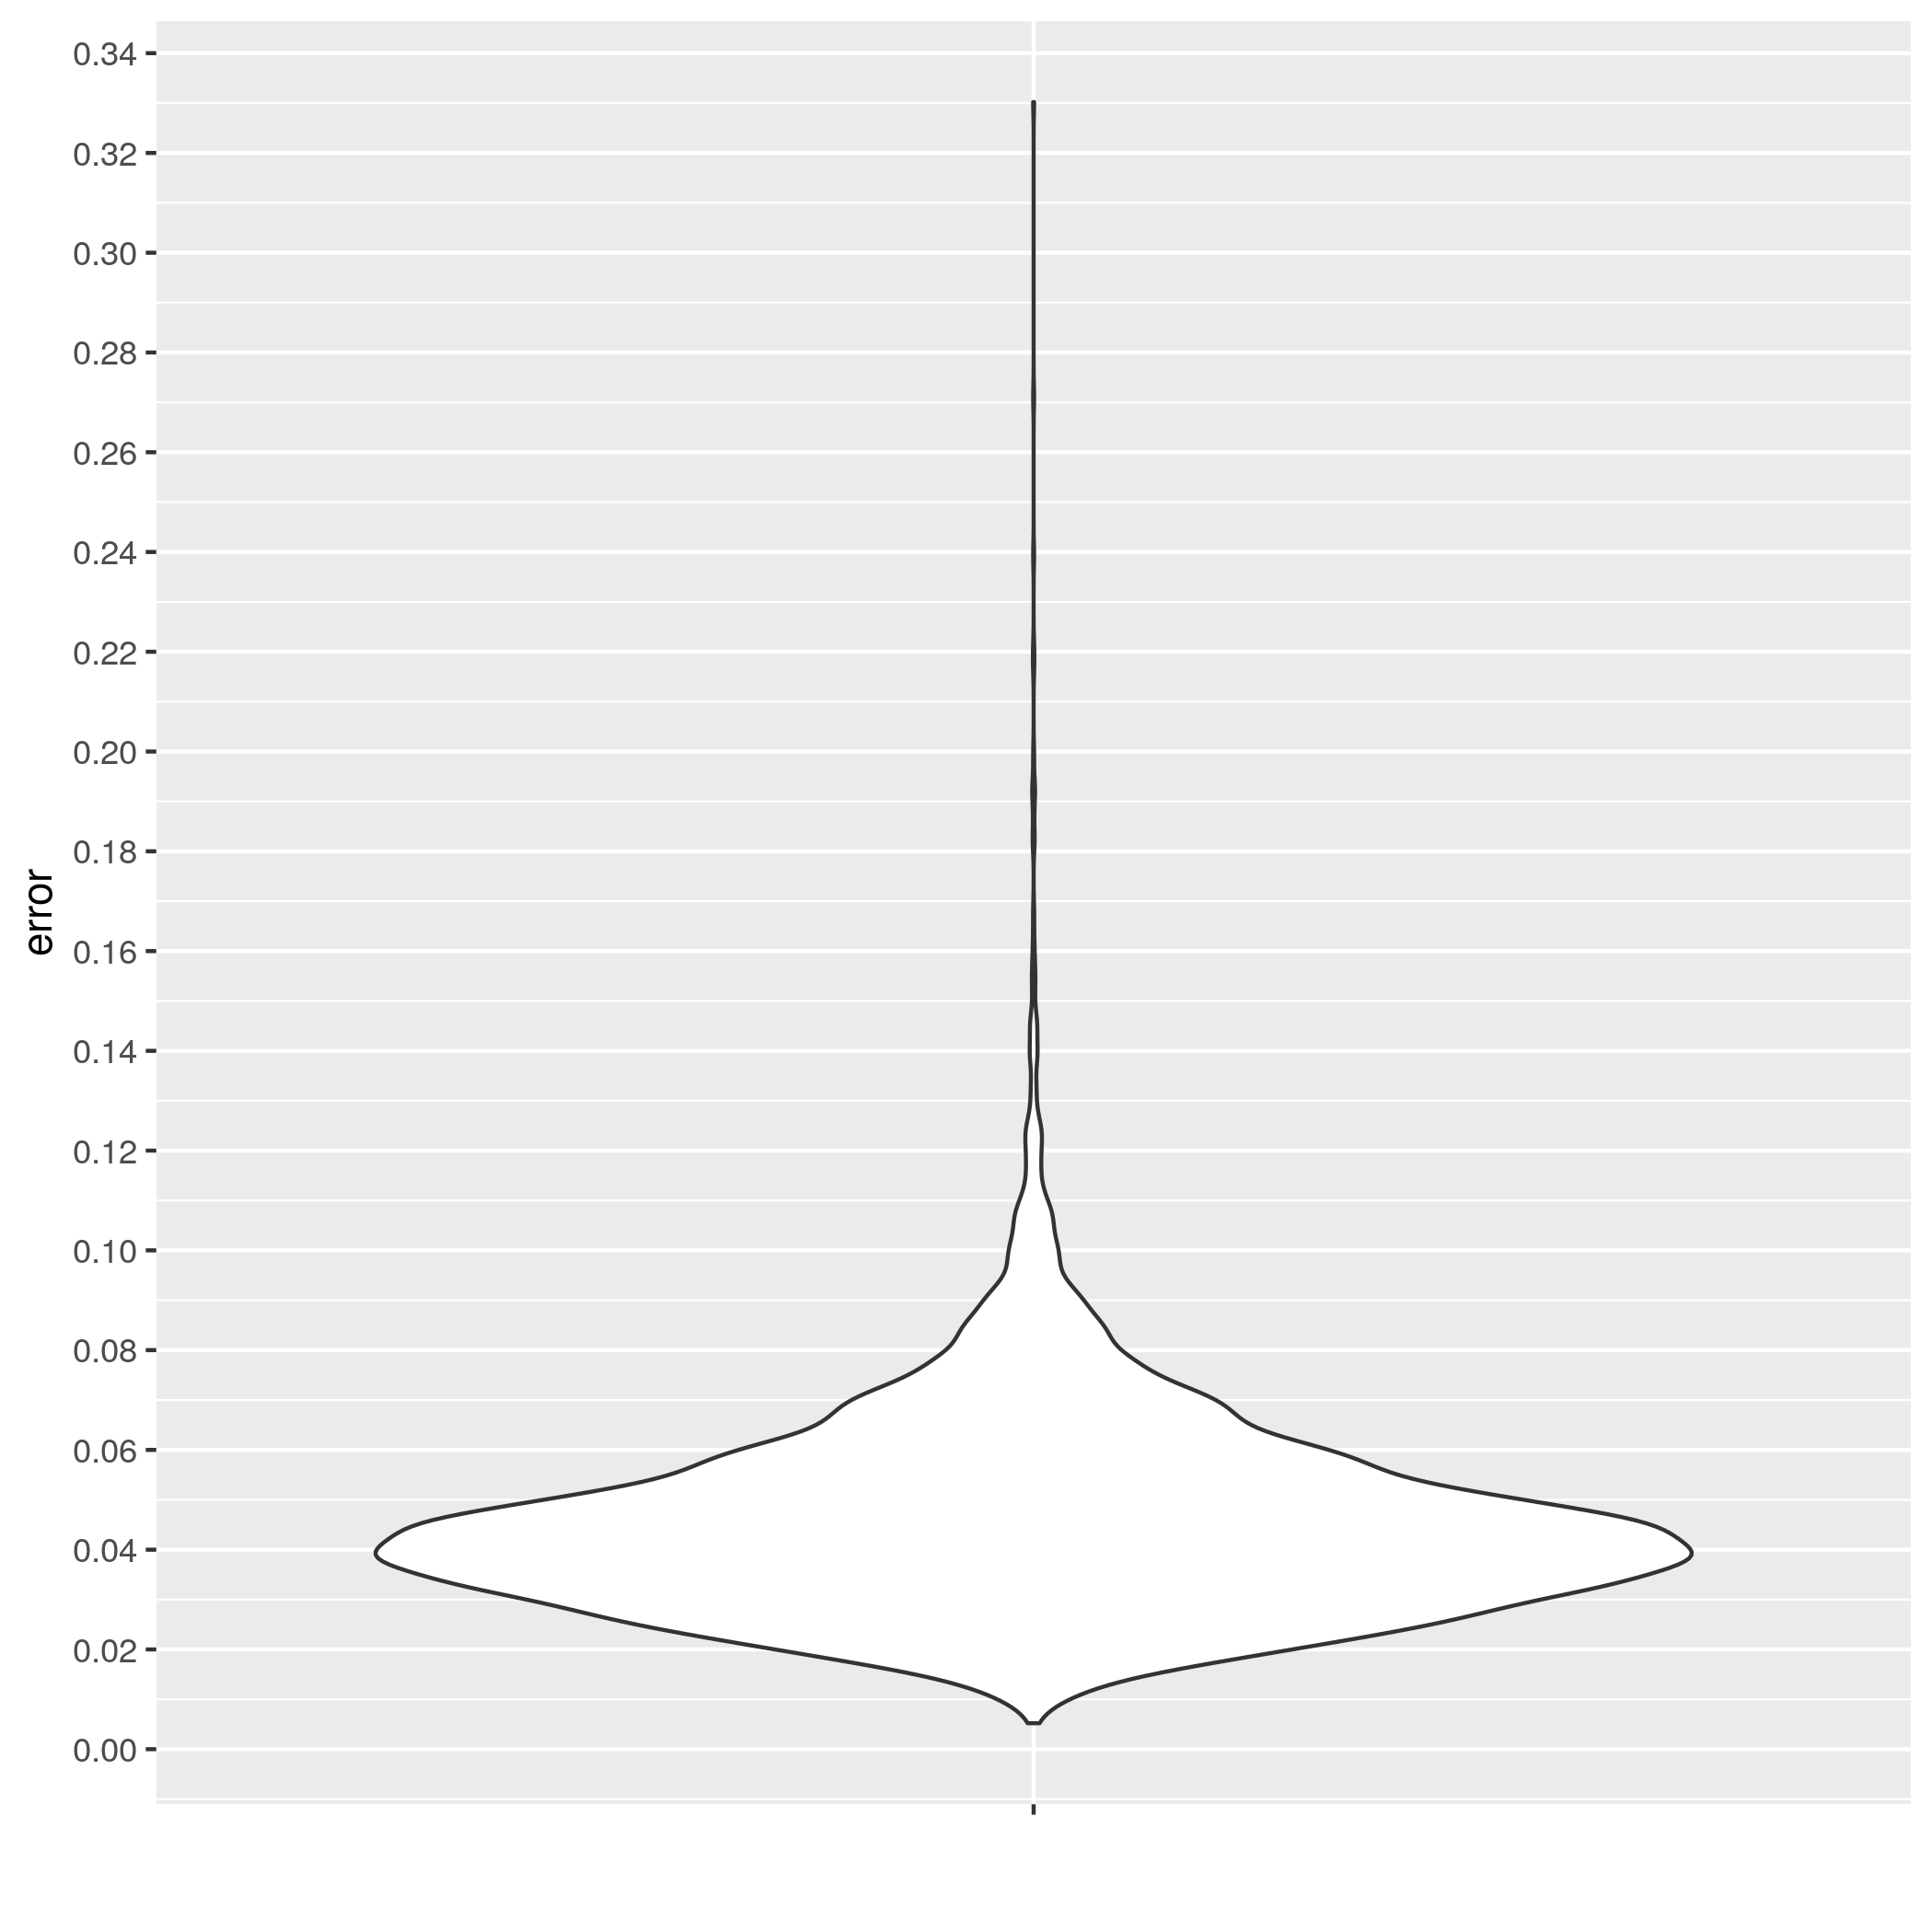
\includegraphics[height=0.2\textheight]{example_3/true_error_violin_best.png}
    };   
    \node[state] (AT) [right of = A, rectangle, node distance=0.8\textheight] {
      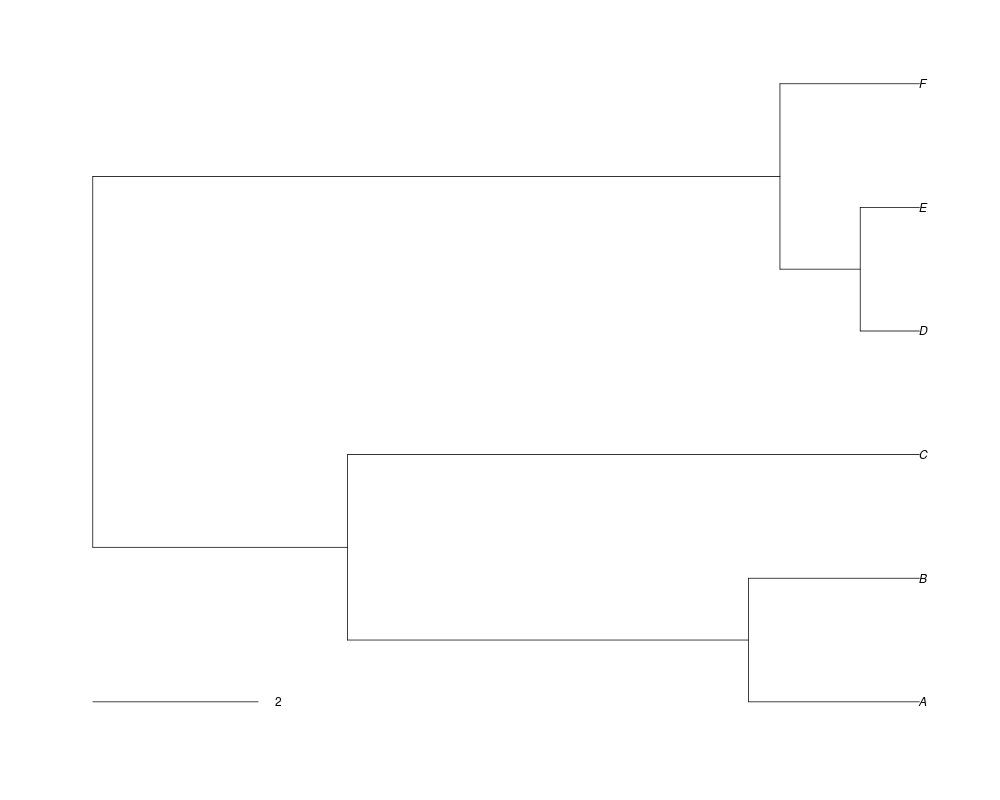
\includegraphics[height=0.2\textheight]{example_3/twin_tree.png}
    };   
    \node[state] (BT) [below of = AT, rectangle] {
      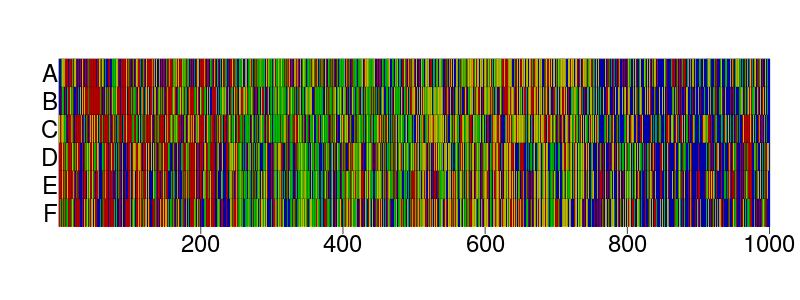
\includegraphics[height=0.13\textheight]{example_3/twin_alignment.png}
    };   
    \node[state] (CTG) [below of = BT, rectangle] {
      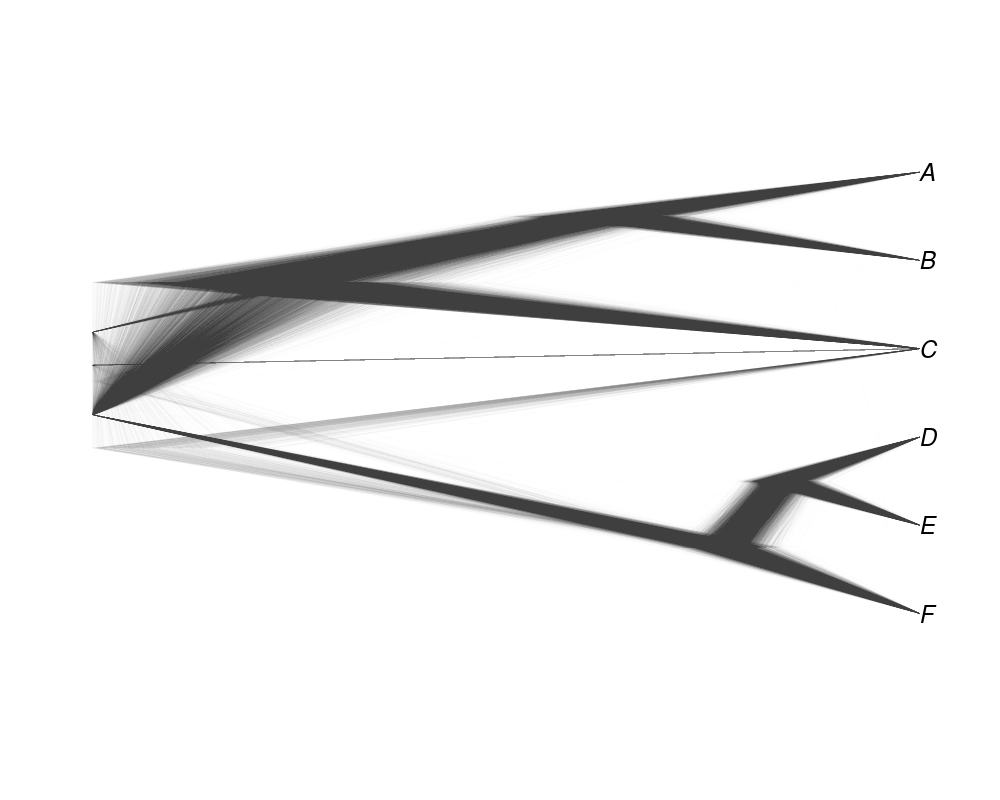
\includegraphics[height=0.2\textheight]{example_3/twin_posterior_gen.png}
    };   
    \node[state] (DTG) [below of = CTG, rectangle] {
      
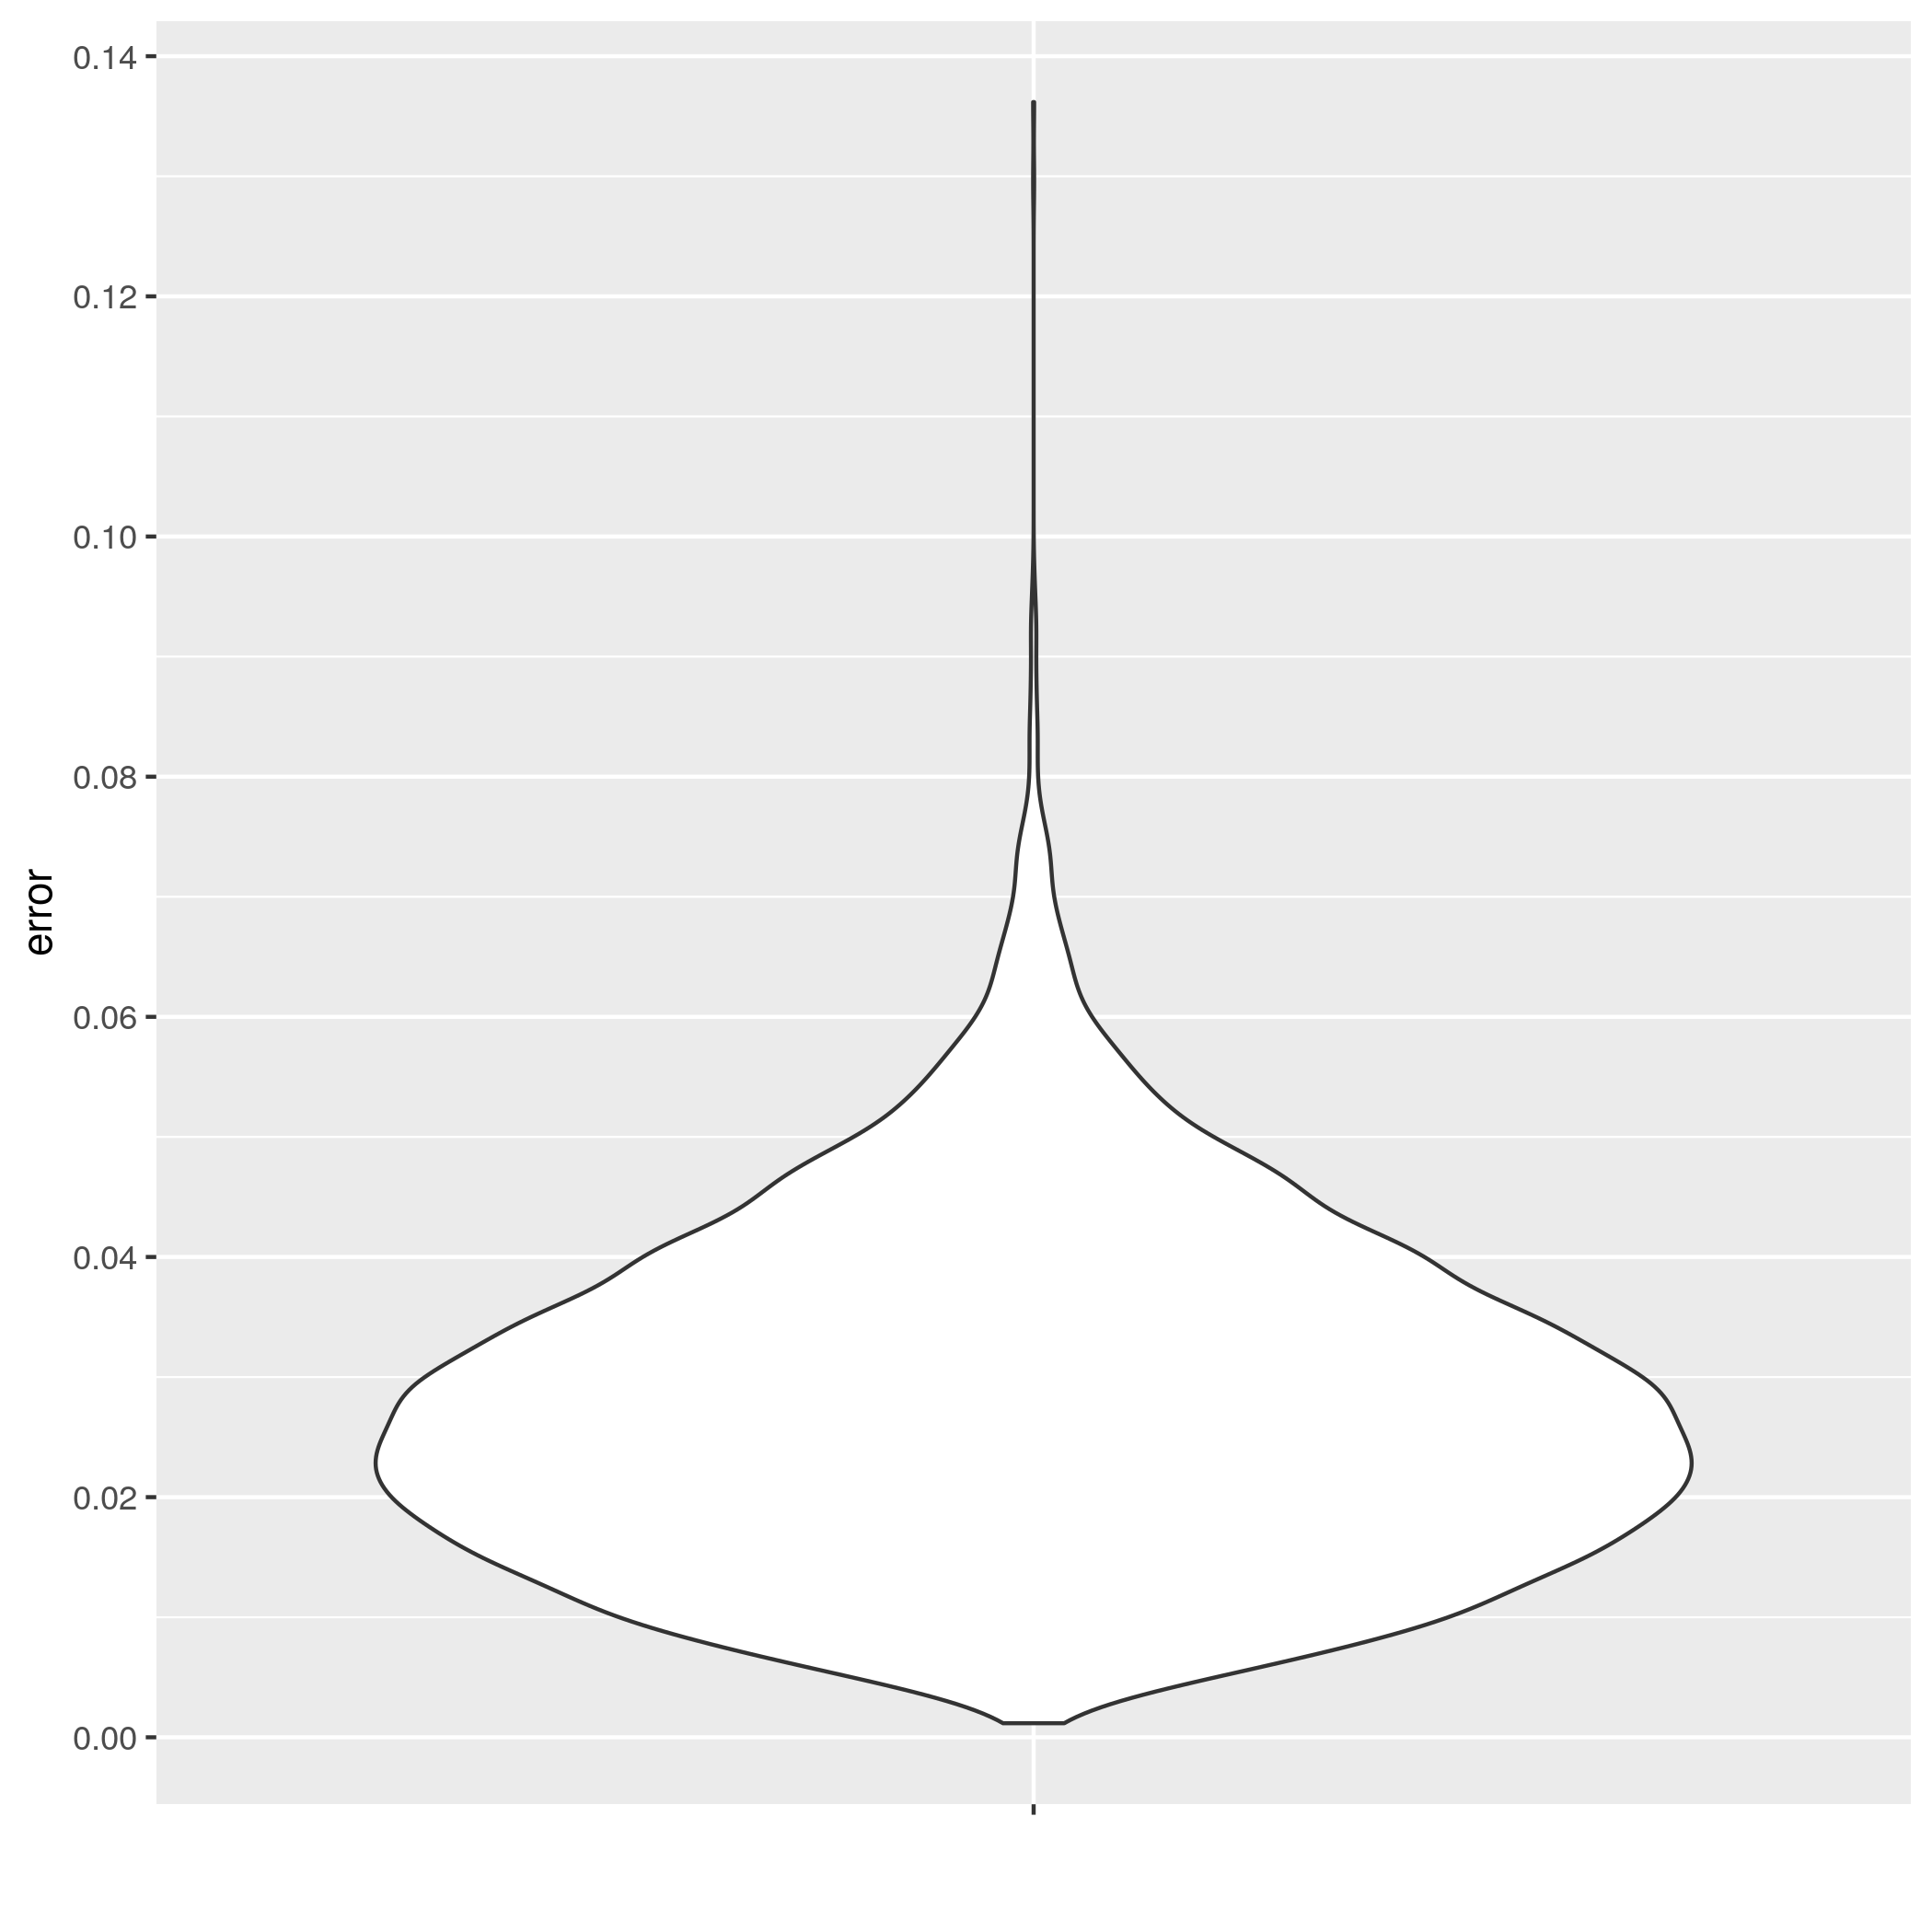
\includegraphics[height=0.2\textheight]{example_3/twin_error_violin_gen.png}
    };   
    \node[state] (CTB) [right of = CTG, rectangle] {
      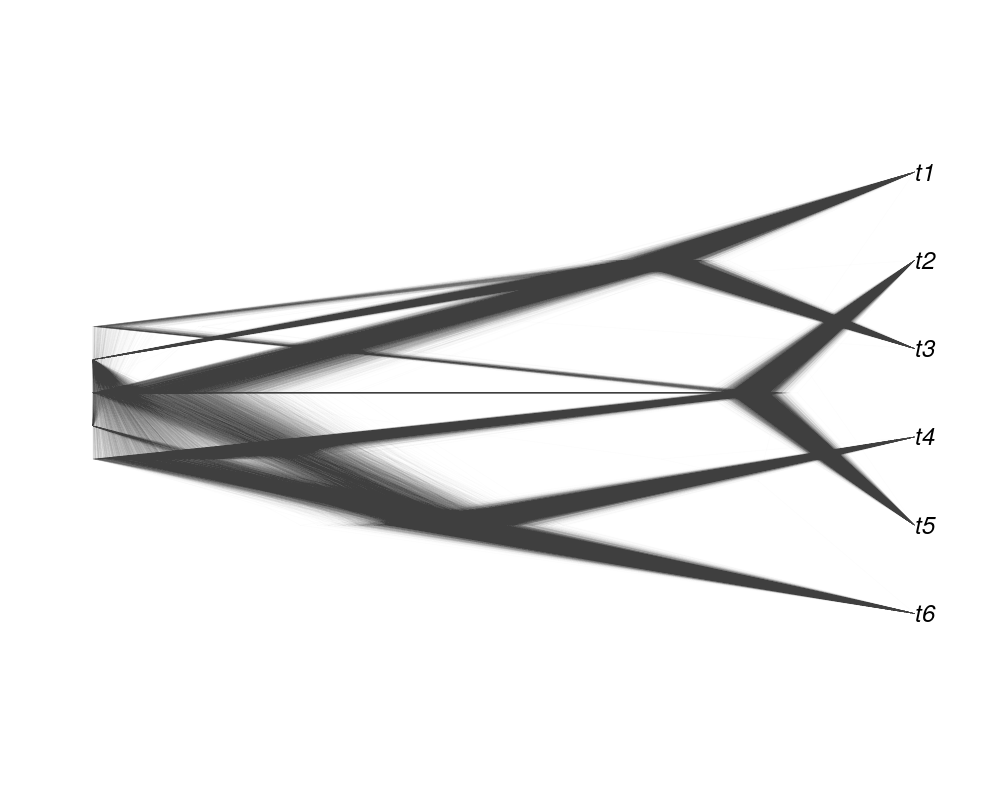
\includegraphics[height=0.2\textheight]{example_3/twin_posterior_best.png}
    };   
    \node[state] (DTB) [below of = CTB, rectangle] {
      
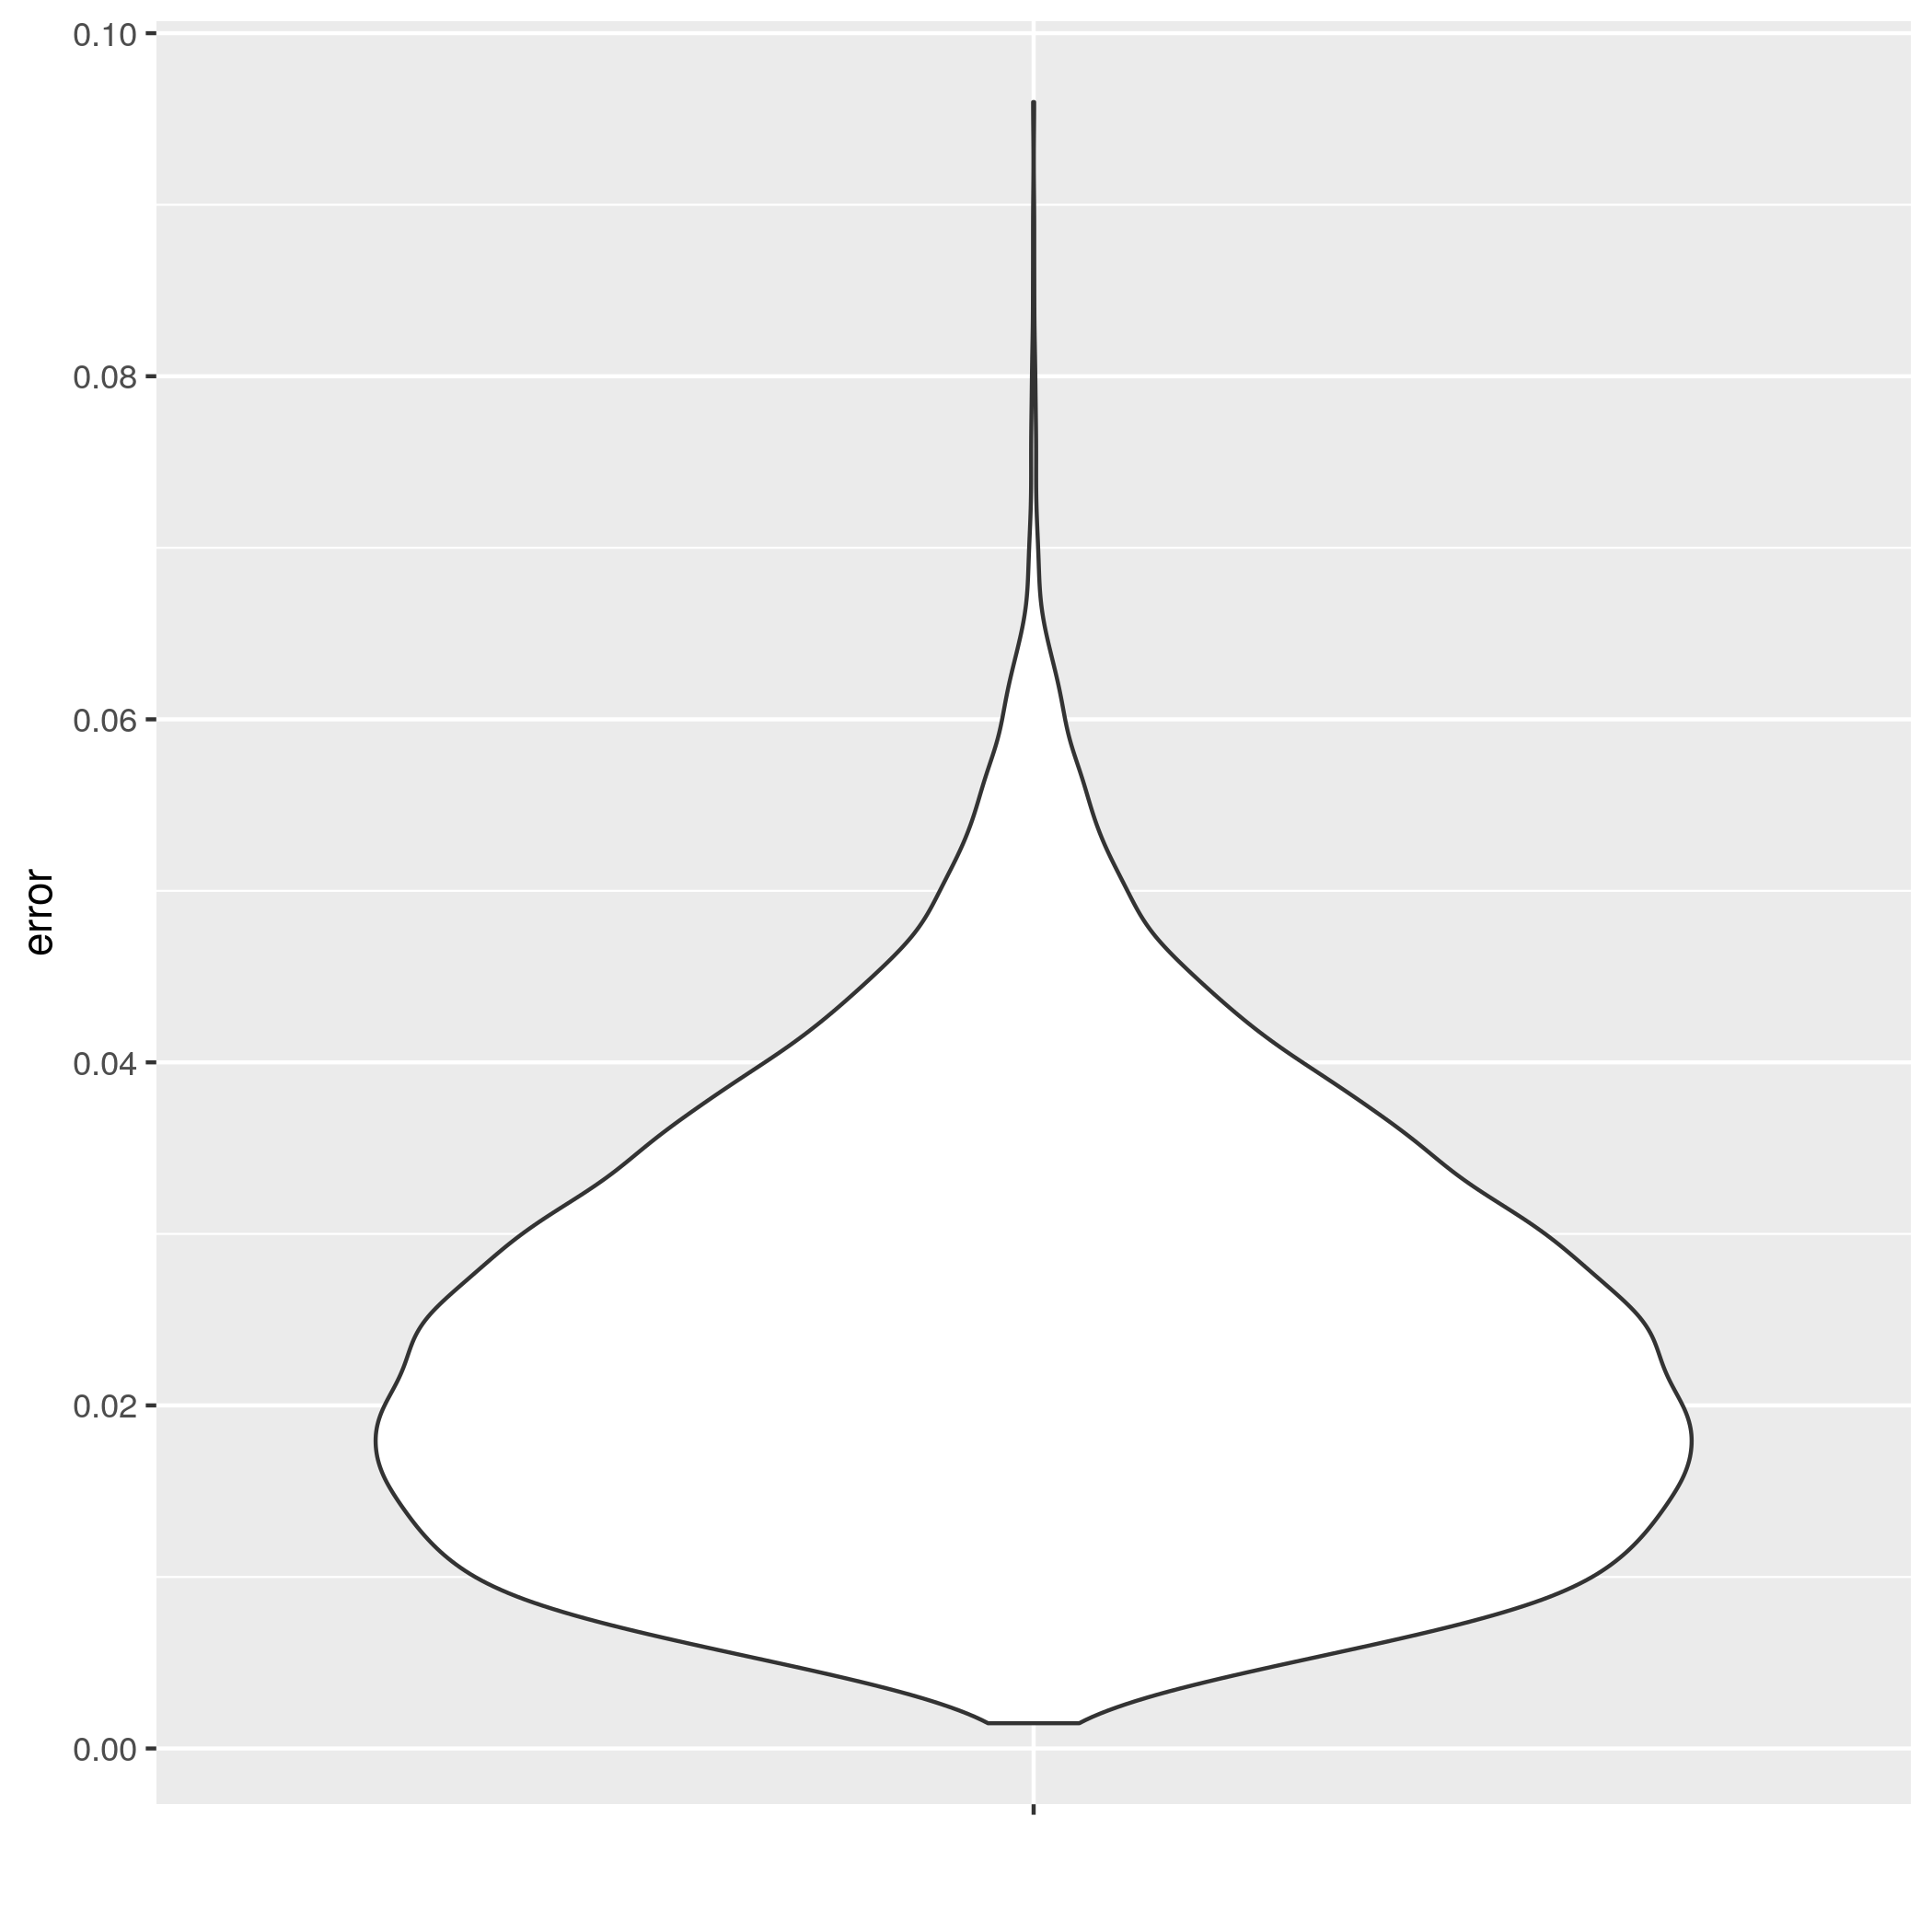
\includegraphics[height=0.2\textheight]{example_3/twin_error_violin_best.png}
    };   
    \path 
      (O) edge [anchor = south] node {} (A)
      (A) edge [anchor = south] node {} (B)
      (B) edge [anchor = south] node {} (CG)
      (CG) edge [anchor = south] node {} (DG)
      (B) edge [anchor = south east] node {} (CB)
      (CB) edge [anchor = south] node {} (DB)
      (A) edge [anchor = east] node {} (AT)
      (AT) edge [anchor = south] node {} (BT)
      (BT) edge [anchor = south east] node {} (CTG)
      (CTG) edge [anchor = south] node {} (DTG)
      (BT) edge [anchor = south] node {} (CTB)
      (CTB) edge [anchor = south] node {} (DTB)
    ; 
    \end{tikzpicture}
  }
  \label{fig:example_3_full_pipeline}
  \caption{Example 5: full pipeline}
\end{figure}
%%%%%%%%%%%%%%%%%%%%%%%%%%%%%%%%%%%%%%%%%%%%%%%%%%%%%%%%%%%%%%%%%%%%%%%%%%%%%%%%

\input{example_3/esses_gen.latex}
% has label tab:esses_example_3_gen

\input{example_3/esses_best.latex}
% has label tab:esses_example_3_best

\input{example_3/esses_twin_gen.latex}
% has label tab:esses_example_3_twin_gen

\input{example_3/esses_twin_best.latex}
% has label tab:esses_example_3_twin_best

\input{example_3/evidence_true.latex}
% has label tab:evidences_example_3

\input{example_3/evidence_twin.latex}
% has label tab:evidences_example_3

\begin{table}
  \begin{tabular}{ | r | c | }
    \hline
    \textbf{ERQ} & \textbf{run-time} \\ 
    \hline
      1 & 00:10:12 \\
      2 & 00:34:10 \\
      3 & 00:24:53 \\
      4 & 01:04:50 \\
      5 & 01:29:40 \\
    \hline
  \end{tabular}
  \caption{
    Time for an example research question to finish.
    Time is in in hh:mm::ss.
  }
  \label{tab:runtime}
\end{table}






%%%%%%%%%%%%%%%%%%%%%%%%%%%%%%%%%%%%%%%%%%%%%%%%%%%%%%%%%%%%%%%%%%%%%%%%%%%%%%%%
\subsection{Example 6}
%%%%%%%%%%%%%%%%%%%%%%%%%%%%%%%%%%%%%%%%%%%%%%%%%%%%%%%%%%%%%%%%%%%%%%%%%%%%%%%%

%%%%%%%%%%%%%%%%%%%%%%%%%%%%%%%%%%%%%%%%%%%%%%%%%%%%%%%%%%%%%%%%%%%%%%%%%%%%%%%%
\begin{figure}[ht]
  \centering
  \resizebox {0.8\columnwidth} {!} {
    \begin{tikzpicture}[
      ->,>=stealth',shorten >=1pt,auto,
      node distance=0.4\textheight, 
      semithick
    ]   
    \tikzstyle{every state}=[]
    \node[state, draw=none] (O) [] {
    };   
    \node[state] (A) [right of = O, rectangle] {
      \includegraphics[height=0.2\textheight]{example_2/true_tree.png}
    };   
    \node[state] (B) [below of = A, rectangle] {
      \includegraphics[height=0.13\textheight]{example_2/true_alignment.png}
    };   
    \node[state] (CG) [below of = B, rectangle] {
      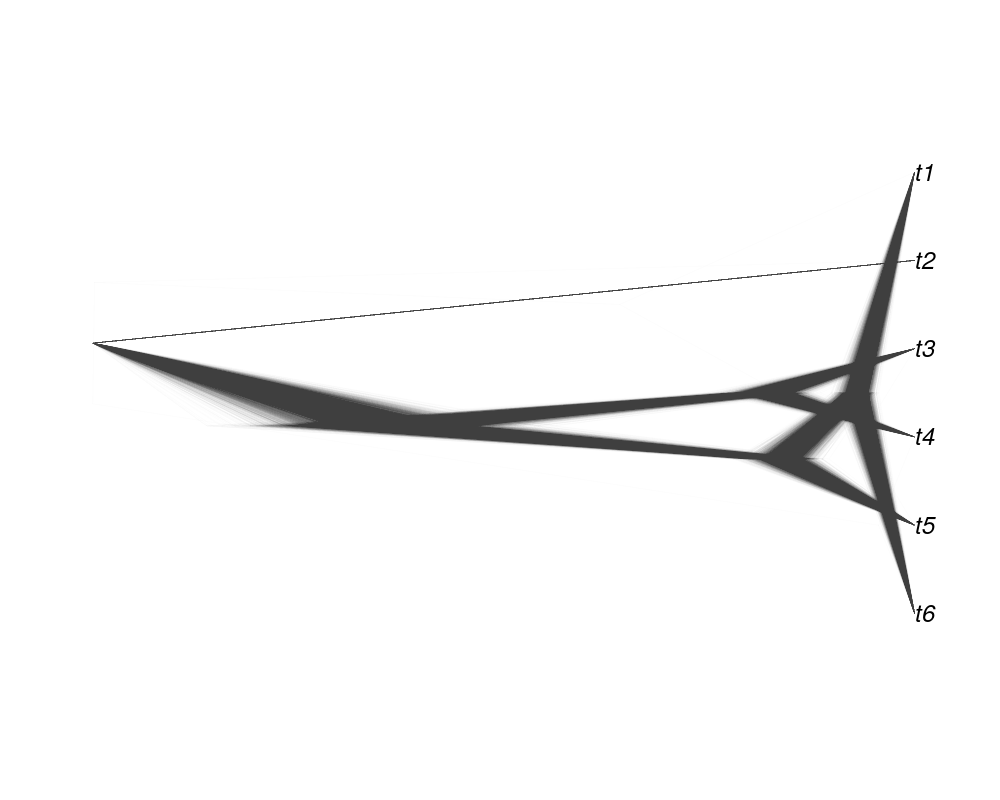
\includegraphics[height=0.2\textheight]{example_2/true_posterior_gen.png}
    };   
    \node[state] (DG) [below of = CG, rectangle] {
      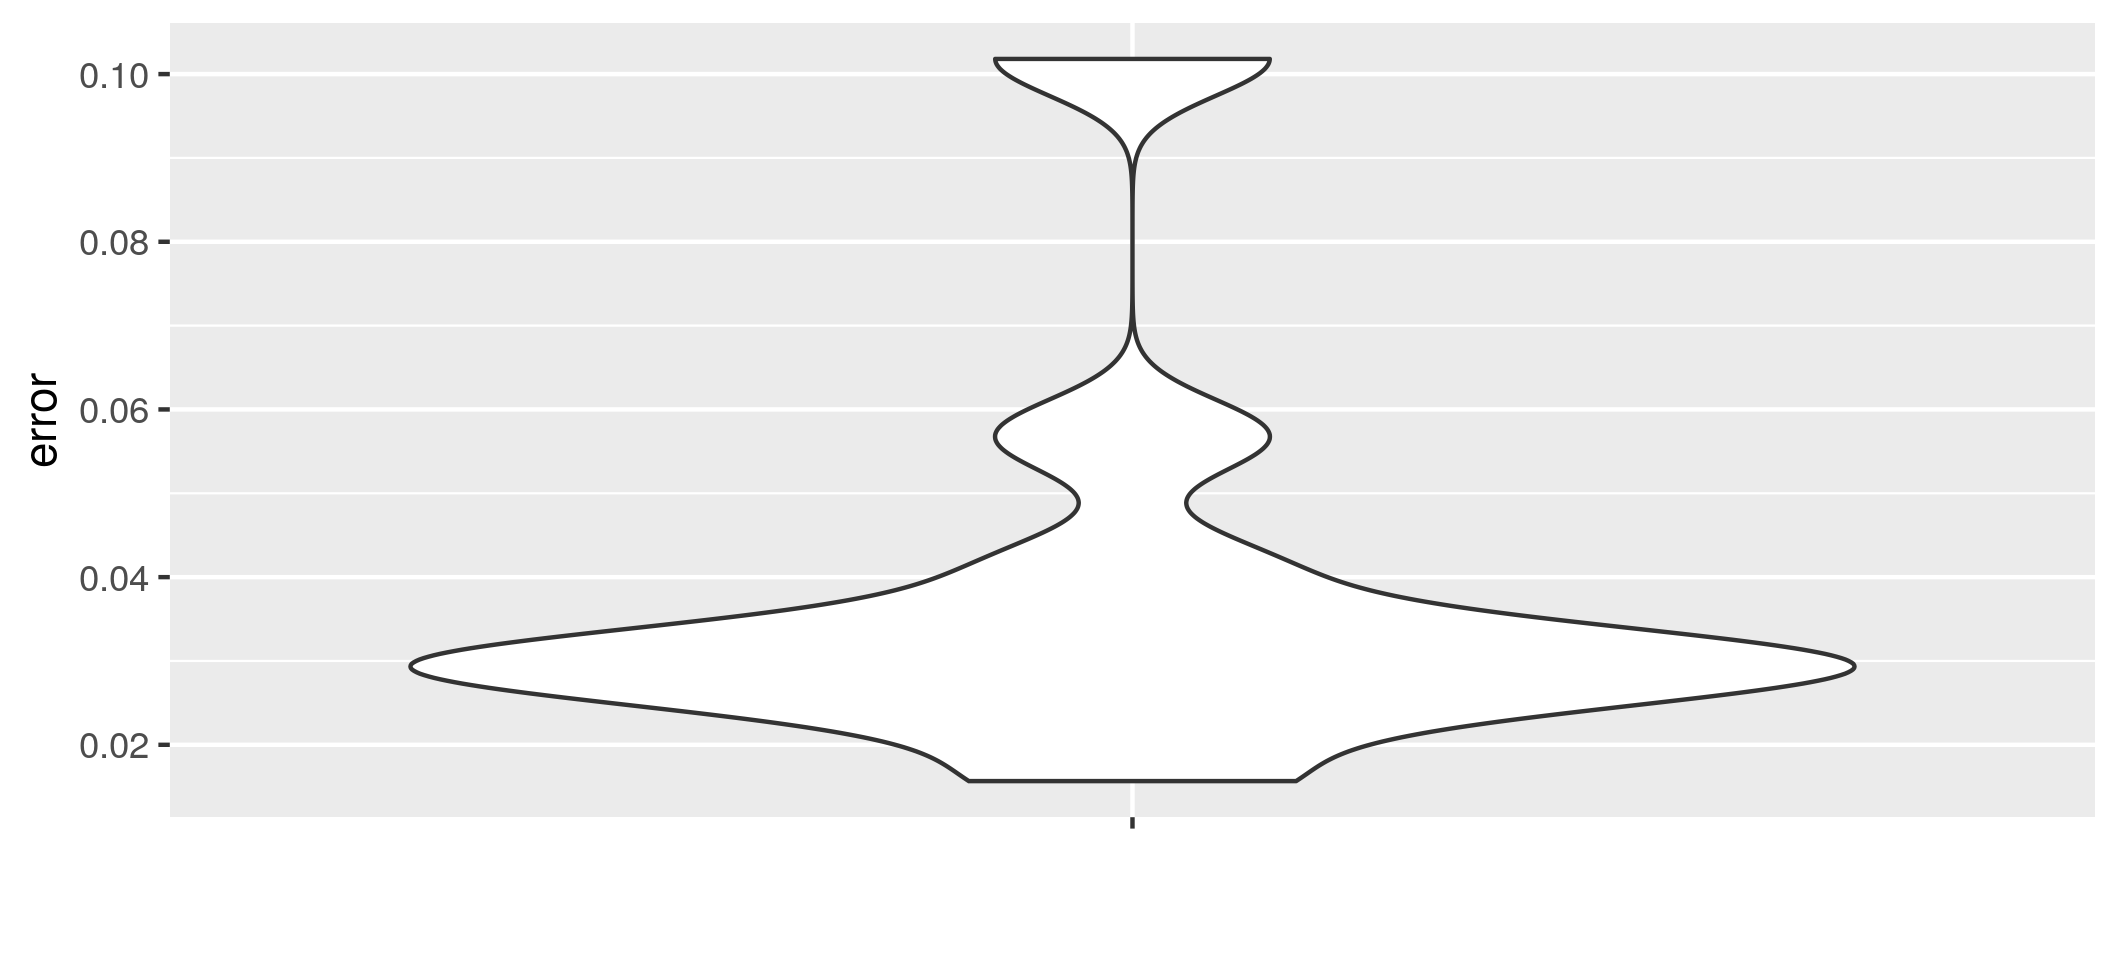
\includegraphics[height=0.2\textheight]{example_2/true_error_violin_gen.png}
    };   
    \node[state] (CB) [right of = C, rectangle] {
      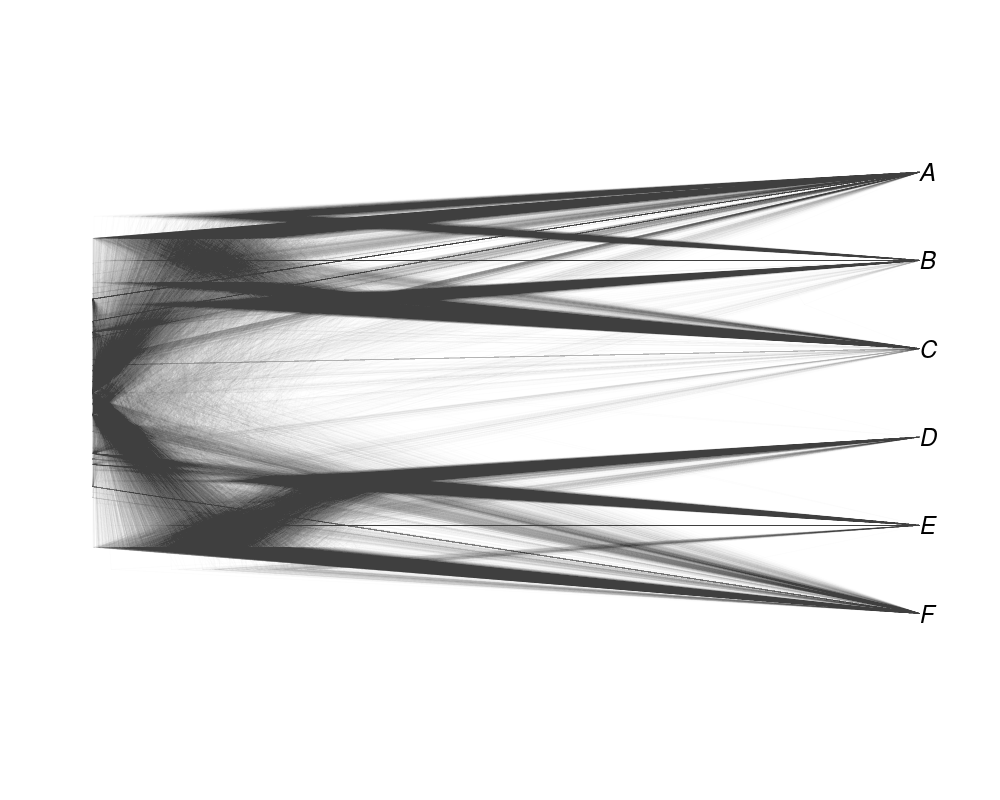
\includegraphics[height=0.2\textheight]{example_2/true_posterior_best.png}
    };   
    \node[state] (DB) [below of = CB, rectangle] {
      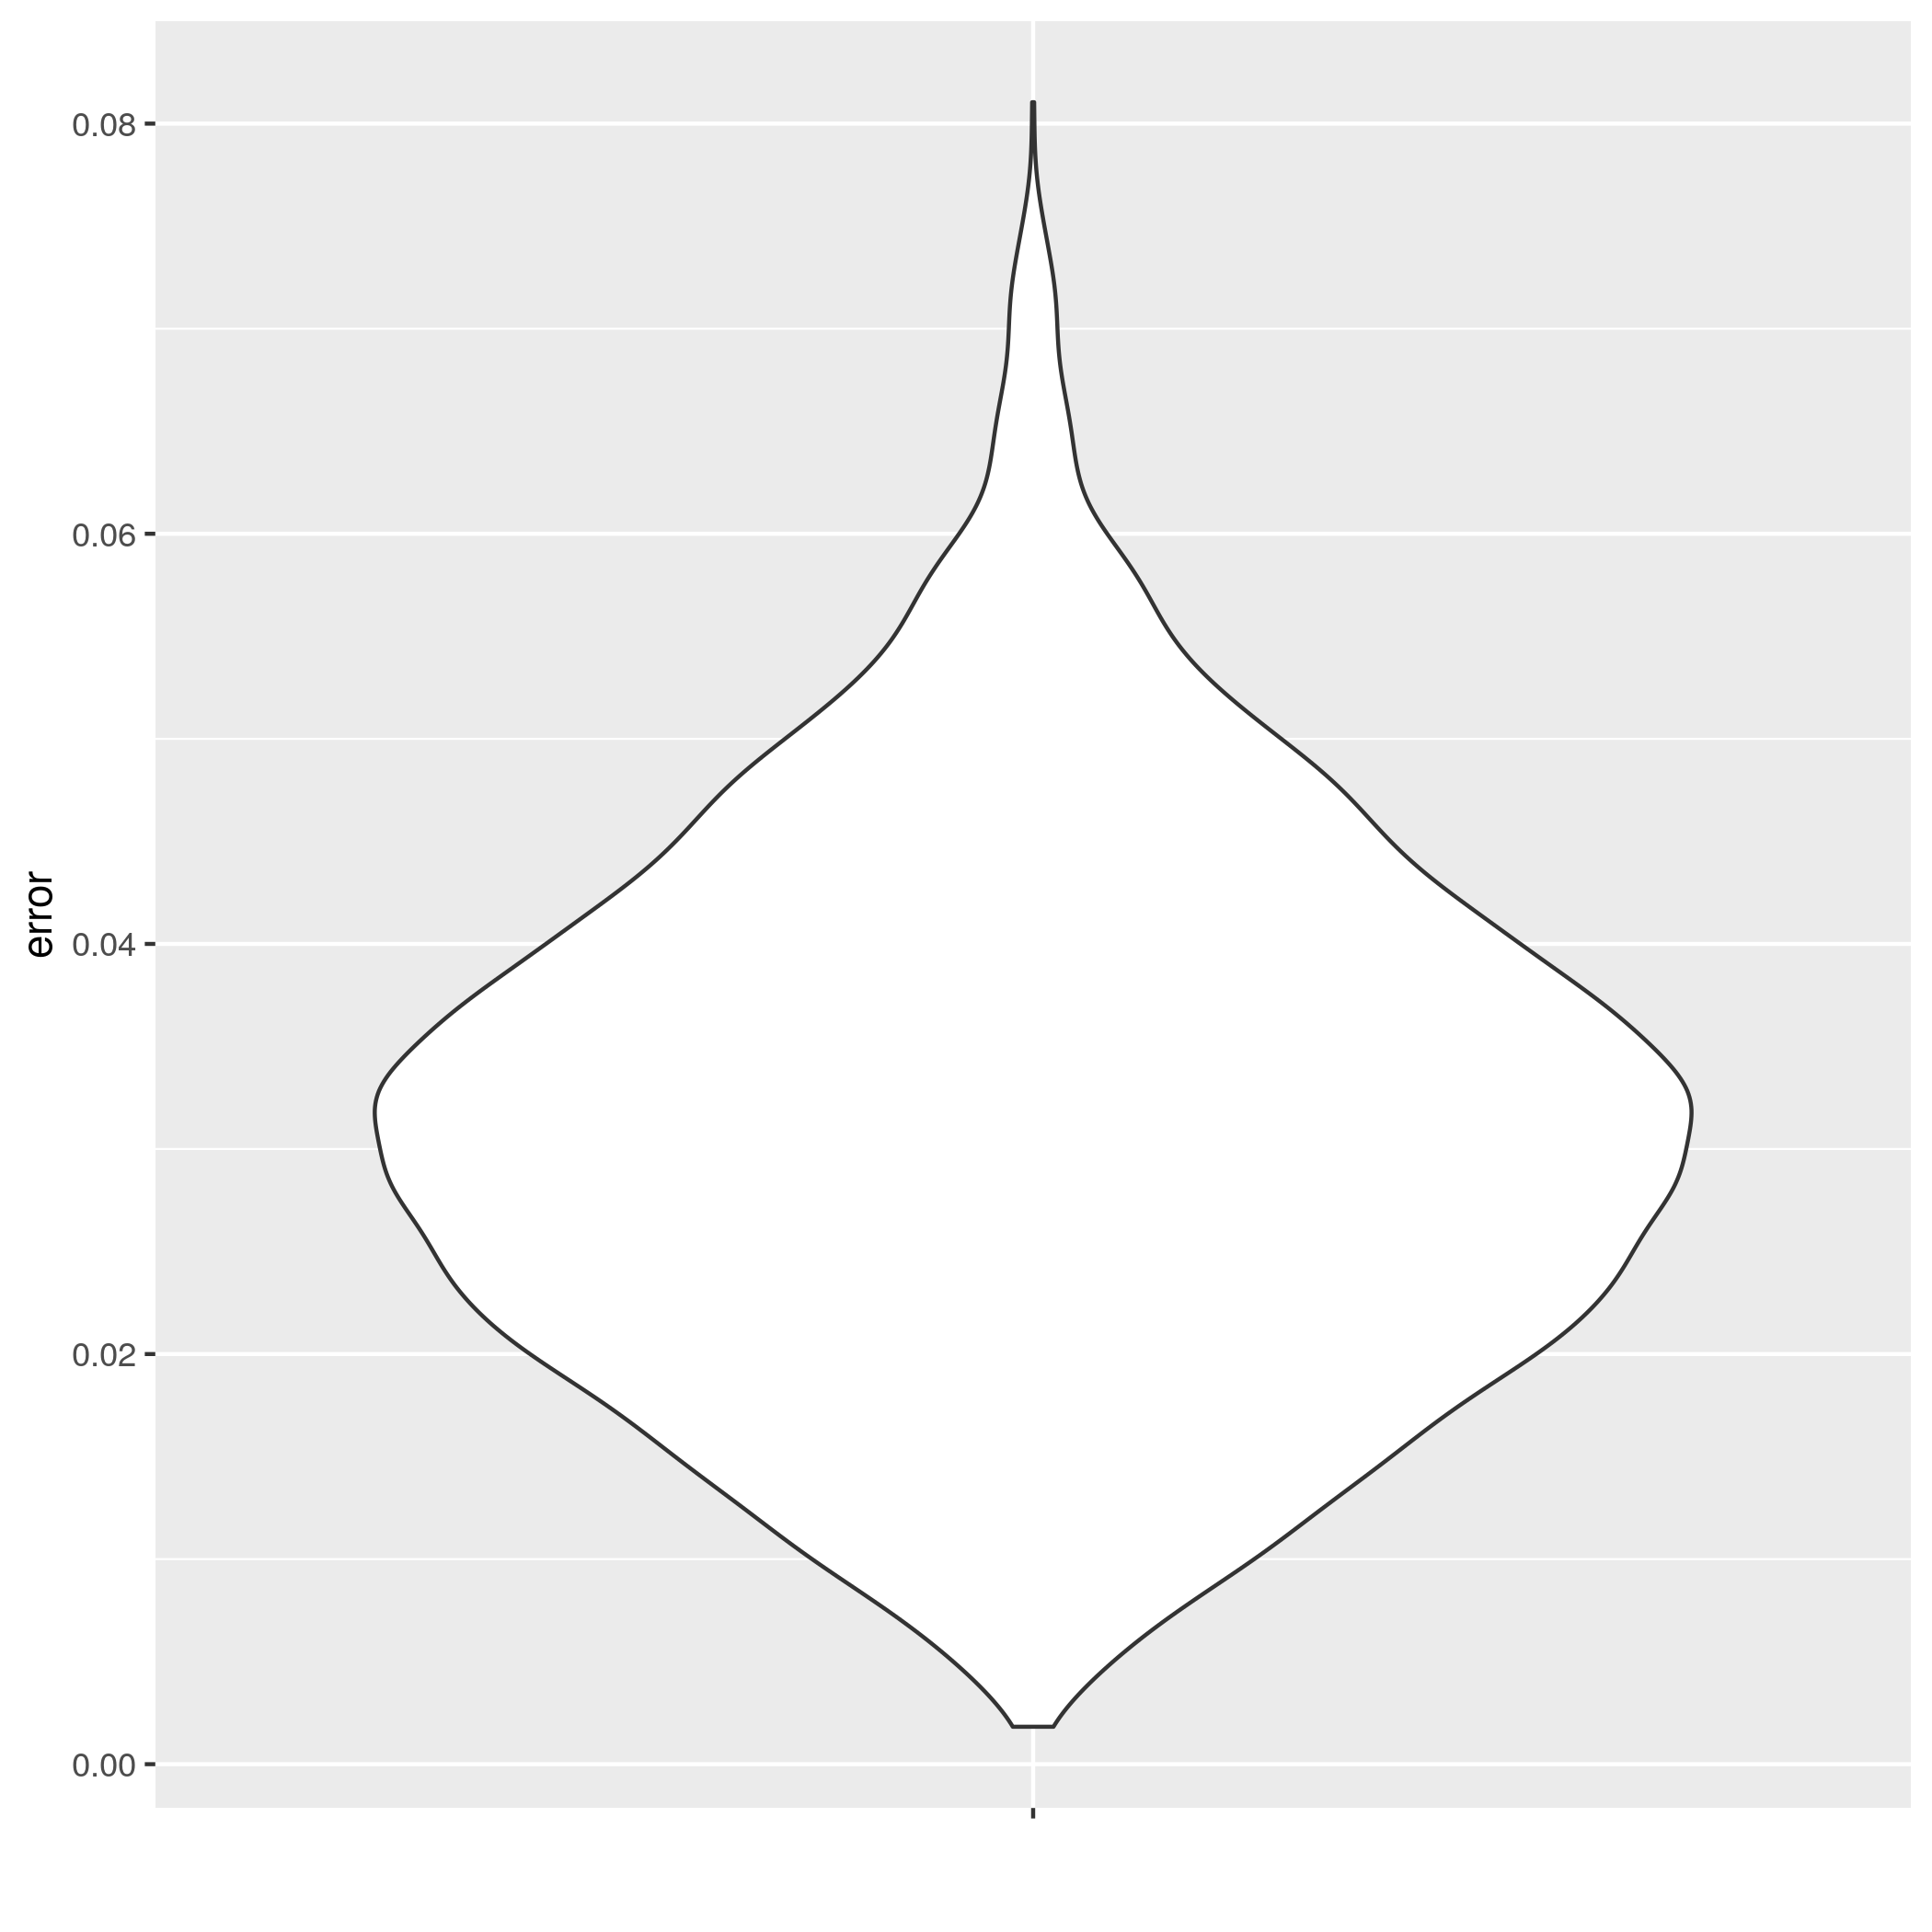
\includegraphics[height=0.2\textheight]{example_2/true_error_violin_best.png}
    };   
    \path 
      (O) edge [anchor = south] node {} (A)
      (A) edge [anchor = south] node {} (B)
      (B) edge [anchor = south] node {} (CG)
      (CG) edge [anchor = south] node {} (DG)
      (B) edge [anchor = south east] node {} (CB)
      (CB) edge [anchor = south] node {} (DB)
    ; 
    \end{tikzpicture}
  }
  \label{fig:example_2_full_pipeline}
  \caption{Example 6: full pipeline}
\end{figure}
%%%%%%%%%%%%%%%%%%%%%%%%%%%%%%%%%%%%%%%%%%%%%%%%%%%%%%%%%%%%%%%%%%%%%%%%%%%%%%%%

\input{example_2/esses_gen.latex}
% has label tab:esses_example_2_gen

\input{example_2/esses_best.latex}
% has label tab:esses_example_2_best

\input{example_2/evidence_true.latex}
% has label tab:evidences_example_2

\begin{table}
  \begin{tabular}{ | r | c | }
    \hline
    \textbf{ERQ} & \textbf{run-time} \\ 
    \hline
      1 & 00:10:12 \\
      2 & 00:34:10 \\
      3 & 00:24:53 \\
      4 & 01:04:50 \\
      5 & 01:29:40 \\
    \hline
  \end{tabular}
  \caption{
    Time for an example research question to finish.
    Time is in in hh:mm::ss.
  }
  \label{tab:runtime}
\end{table}


\end{document}
